\documentclass[reqno,10pt,a4paper,oneside]{amsart}

\usepackage{amsmath,geometry}
\usepackage{amssymb,mathpartir,mathtools}
\usepackage{latexsym}
\usepackage{amsthm}
 \usepackage[show]{ed}
\usepackage{leftidx}
\usepackage{tikz}

\usepackage[all]{xy}
\newcommand{\xycenter}[1]{\vcenter{\hbox{\xymatrix{#1}}}}
\SelectTips{cm}{}

\message{<Paul Taylor's Proof Trees, 2 August 1996>}
%% Build proof tree for Natural Deduction, Sequent Calculus, etc.
%% WITH SHORTENING OF PROOF RULES!
%% Paul Taylor, begun 10 Oct 1989
%% *** THIS IS ONLY A PRELIMINARY VERSION AND THINGS MAY CHANGE! ***
%%
%% 2 Aug 1996: fixed \mscount and \proofdotnumber
%%
%%      \prooftree
%%              hyp1            produces:
%%              hyp2
%%              hyp3            hyp1    hyp2    hyp3
%%      \justifies              -------------------- rulename
%%              concl                   concl
%%      \thickness=0.08em
%%      \shiftright 2em
%%      \using
%%              rulename
%%      \endprooftree
%%
%% where the hypotheses may be similar structures or just formulae.
%%
%% To get a vertical string of dots instead of the proof rule, do
%%
%%      \prooftree                      which produces:
%%              [hyp]
%%      \using                                  [hyp]
%%              name                              .
%%      \proofdotseparation=1.2ex                 .name
%%      \proofdotnumber=4                         .
%%      \leadsto                                  .
%%              concl                           concl
%%      \endprooftree
%%
%% Within a prooftree, \[ and \] may be used instead of \prooftree and
%% \endprooftree; this is not permitted at the outer level because it
%% conflicts with LaTeX. Also,
%%      \Justifies
%% produces a double line. In LaTeX you can use \begin{prooftree} and
%% \end{prootree} at the outer level (however this will not work for the inner
%% levels, but in any case why would you want to be so verbose?).
%%
%% All of of the keywords except \prooftree and \endprooftree are optional
%% and may appear in any order. They may also be combined in \newcommand's
%% eg "\def\Cut{\using\sf cut\thickness.08em\justifies}" with the abbreviation
%% "\prooftree hyp1 hyp2 \Cut \concl \endprooftree". This is recommended and
%% some standard abbreviations will be found at the end of this file.
%%
%% \thickness specifies the breadth of the rule in any units, although
%% font-relative units such as "ex" or "em" are preferable.
%% It may optionally be followed by "=".
%% \proofrulebreadth=.08em or \setlength\proofrulebreadth{.08em} may also be
%% used either in place of \thickness or globally; the default is 0.04em.
%% \proofdotseparation and \proofdotnumber control the size of the
%% string of dots
%%
%% If proof trees and formulae are mixed, some explicit spacing is needed,
%% but don't put anything to the left of the left-most (or the right of
%% the right-most) hypothesis, or put it in braces, because this will cause
%% the indentation to be lost.
%%
%% By default the conclusion is centered wrt the left-most and right-most
%% immediate hypotheses (not their proofs); \shiftright or \shiftleft moves
%% it relative to this position. (Not sure about this specification or how
%% it should affect spreading of proof tree.)
%
% global assignments to dimensions seem to have the effect of stretching
% diagrams horizontally.
%
%%==========================================================================

\def\introrule{{\cal I}}\def\elimrule{{\cal E}}%%
\def\andintro{\using{\land}\introrule\justifies}%%
\def\impelim{\using{\Rightarrow}\elimrule\justifies}%%
\def\allintro{\using{\forall}\introrule\justifies}%%
\def\allelim{\using{\forall}\elimrule\justifies}%%
\def\falseelim{\using{\bot}\elimrule\justifies}%%
\def\existsintro{\using{\exists}\introrule\justifies}%%

%% #1 is meant to be 1 or 2 for the first or second formula
\def\andelim#1{\using{\land}#1\elimrule\justifies}%%
\def\orintro#1{\using{\lor}#1\introrule\justifies}%%

%% #1 is meant to be a label corresponding to the discharged hypothesis/es
\def\impintro#1{\using{\Rightarrow}\introrule_{#1}\justifies}%%
\def\orelim#1{\using{\lor}\elimrule_{#1}\justifies}%%
\def\existselim#1{\using{\exists}\elimrule_{#1}\justifies}

%%==========================================================================

\newdimen\proofrulebreadth \proofrulebreadth=.05em
\newdimen\proofdotseparation \proofdotseparation=1.25ex
\newdimen\proofrulebaseline \proofrulebaseline=2ex
\newcount\proofdotnumber \proofdotnumber=3
\let\then\relax
\def\hfi{\hskip0pt plus.0001fil}
\mathchardef\squigto="3A3B
%
% flag where we are
\newif\ifinsideprooftree\insideprooftreefalse
\newif\ifonleftofproofrule\onleftofproofrulefalse
\newif\ifproofdots\proofdotsfalse
\newif\ifdoubleproof\doubleprooffalse
\let\wereinproofbit\relax
%
% dimensions and boxes of bits
\newdimen\shortenproofleft
\newdimen\shortenproofright
\newdimen\proofbelowshift
\newbox\proofabove
\newbox\proofbelow
\newbox\proofrulename
%
% miscellaneous commands for setting values
\def\shiftproofbelow{\let\next\relax\afterassignment\setshiftproofbelow\dimen0 }
\def\shiftproofbelowneg{\def\next{\multiply\dimen0 by-1 }%
\afterassignment\setshiftproofbelow\dimen0 }
\def\setshiftproofbelow{\next\proofbelowshift=\dimen0 }
\def\setproofrulebreadth{\proofrulebreadth}

%=============================================================================
\def\prooftree{% NESTED ZERO (\ifonleftofproofrule)
%
% first find out whether we're at the left-hand end of a proof rule
\ifnum  \lastpenalty=1
\then   \unpenalty
\else   \onleftofproofrulefalse
\fi
%
% some space on left (except if we're on left, and no infinity for outermost)
\ifonleftofproofrule
\else   \ifinsideprooftree
        \then   \hskip.5em plus1fil
        \fi
\fi
%
% begin our proof tree environment
\bgroup% NESTED ONE (\proofbelow, \proofrulename, \proofabove,
%               \shortenproofleft, \shortenproofright, \proofrulebreadth)
\setbox\proofbelow=\hbox{}\setbox\proofrulename=\hbox{}%
\let\justifies\proofover\let\leadsto\proofoverdots\let\Justifies\proofoverdbl
\let\using\proofusing\let\[\prooftree
\ifinsideprooftree\let\]\endprooftree\fi
\proofdotsfalse\doubleprooffalse
\let\thickness\setproofrulebreadth
\let\shiftright\shiftproofbelow \let\shift\shiftproofbelow
\let\shiftleft\shiftproofbelowneg
\let\ifwasinsideprooftree\ifinsideprooftree
\insideprooftreetrue
%
% now begin to set the top of the rule (definitions local to it)
\setbox\proofabove=\hbox\bgroup$\displaystyle % NESTED TWO
\let\wereinproofbit\prooftree
%
% these local variables will be copied out:
\shortenproofleft=0pt \shortenproofright=0pt \proofbelowshift=0pt
%
% flags to enable inner proof tree to detect if on left:
\onleftofproofruletrue\penalty1
}

%=============================================================================
% end whatever box and copy crucial values out of it
\def\eproofbit{% NESTED TWO
%
% various hacks applicable to hypothesis list 
\ifx    \wereinproofbit\prooftree
\then   \ifcase \lastpenalty
        \then   \shortenproofright=0pt  % 0: some other object, no indentation
        \or     \unpenalty\hfil         % 1: empty hypotheses, just glue
        \or     \unpenalty\unskip       % 2: just had a tree, remove glue
        \else   \shortenproofright=0pt  % eh?
        \fi
\fi
%
% pass out crucial values from scope
\global\dimen0=\shortenproofleft
\global\dimen1=\shortenproofright
\global\dimen2=\proofrulebreadth
\global\dimen3=\proofbelowshift
\global\dimen4=\proofdotseparation
\global\count255=\proofdotnumber
%
% end the box
$\egroup  % NESTED ONE
%
% restore the values
\shortenproofleft=\dimen0
\shortenproofright=\dimen1
\proofrulebreadth=\dimen2
\proofbelowshift=\dimen3
\proofdotseparation=\dimen4
\proofdotnumber=\count255
}

%=============================================================================
\def\proofover{% NESTED TWO
\eproofbit % NESTED ONE
\setbox\proofbelow=\hbox\bgroup % NESTED TWO
\let\wereinproofbit\proofover
$\displaystyle
}%
%
%=============================================================================
\def\proofoverdbl{% NESTED TWO
\eproofbit % NESTED ONE
\doubleprooftrue
\setbox\proofbelow=\hbox\bgroup % NESTED TWO
\let\wereinproofbit\proofoverdbl
$\displaystyle
}%
%
%=============================================================================
\def\proofoverdots{% NESTED TWO
\eproofbit % NESTED ONE
\proofdotstrue
\setbox\proofbelow=\hbox\bgroup % NESTED TWO
\let\wereinproofbit\proofoverdots
$\displaystyle
}%
%
%=============================================================================
\def\proofusing{% NESTED TWO
\eproofbit % NESTED ONE
\setbox\proofrulename=\hbox\bgroup % NESTED TWO
\let\wereinproofbit\proofusing
\kern0.3em$
}

%=============================================================================
\def\endprooftree{% NESTED TWO
\eproofbit % NESTED ONE
% \dimen0 =     length of proof rule
% \dimen1 =     indentation of conclusion wrt rule
% \dimen2 =     new \shortenproofleft, ie indentation of conclusion
% \dimen3 =     new \shortenproofright, ie
%                space on right of conclusion to end of tree
% \dimen4 =     space on right of conclusion below rule
  \dimen5 =0pt% spread of hypotheses
% \dimen6, \dimen7 = height & depth of rule
%
% length of rule needed by proof above
\dimen0=\wd\proofabove \advance\dimen0-\shortenproofleft
\advance\dimen0-\shortenproofright
%
% amount of spare space below
\dimen1=.5\dimen0 \advance\dimen1-.5\wd\proofbelow
\dimen4=\dimen1
\advance\dimen1\proofbelowshift \advance\dimen4-\proofbelowshift
%
% conclusion sticks out to left of immediate hypotheses
\ifdim  \dimen1<0pt
\then   \advance\shortenproofleft\dimen1
        \advance\dimen0-\dimen1
        \dimen1=0pt
%       now it sticks out to left of tree!
        \ifdim  \shortenproofleft<0pt
        \then   \setbox\proofabove=\hbox{%
                        \kern-\shortenproofleft\unhbox\proofabove}%
                \shortenproofleft=0pt
        \fi
\fi
%
% and to the right
\ifdim  \dimen4<0pt
\then   \advance\shortenproofright\dimen4
        \advance\dimen0-\dimen4
        \dimen4=0pt
\fi
%
% make sure enough space for label
\ifdim  \shortenproofright<\wd\proofrulename
\then   \shortenproofright=\wd\proofrulename
\fi
%
% calculate new indentations
\dimen2=\shortenproofleft \advance\dimen2 by\dimen1
\dimen3=\shortenproofright\advance\dimen3 by\dimen4
%
% make the rule or dots, with name attached
\ifproofdots
\then
        \dimen6=\shortenproofleft \advance\dimen6 .5\dimen0
        \setbox1=\vbox to\proofdotseparation{\vss\hbox{$\cdot$}\vss}%
        \setbox0=\hbox{%
                \advance\dimen6-.5\wd1
                \kern\dimen6
                $\vcenter to\proofdotnumber\proofdotseparation
                        {\leaders\box1\vfill}$%
                \unhbox\proofrulename}%
\else   \dimen6=\fontdimen22\the\textfont2 % height of maths axis
        \dimen7=\dimen6
        \advance\dimen6by.5\proofrulebreadth
        \advance\dimen7by-.5\proofrulebreadth
        \setbox0=\hbox{%
                \kern\shortenproofleft
                \ifdoubleproof
                \then   \hbox to\dimen0{%
                        $\mathsurround0pt\mathord=\mkern-6mu%
                        \cleaders\hbox{$\mkern-2mu=\mkern-2mu$}\hfill
                        \mkern-6mu\mathord=$}%
                \else   \vrule height\dimen6 depth-\dimen7 width\dimen0
                \fi
                \unhbox\proofrulename}%
        \ht0=\dimen6 \dp0=-\dimen7
\fi
%
% set up to centre outermost tree only
\let\doll\relax
\ifwasinsideprooftree
\then   \let\VBOX\vbox
\else   \ifmmode\else$\let\doll=$\fi
        \let\VBOX\vcenter
\fi
% this \vbox or \vcenter is the actual output:
\VBOX   {\baselineskip\proofrulebaseline \lineskip.2ex
        \expandafter\lineskiplimit\ifproofdots0ex\else-0.6ex\fi
        \hbox   spread\dimen5   {\hfi\unhbox\proofabove\hfi}%
        \hbox{\box0}%
        \hbox   {\kern\dimen2 \box\proofbelow}}\doll%
%
% pass new indentations out of scope
\global\dimen2=\dimen2
\global\dimen3=\dimen3
\egroup % NESTED ZERO
\ifonleftofproofrule
\then   \shortenproofleft=\dimen2
\fi
\shortenproofright=\dimen3
%
% some space on right and flag we've just made a tree
\onleftofproofrulefalse
\ifinsideprooftree
\then   \hskip.5em plus 1fil \penalty2
\fi
}

%==========================================================================
% IDEAS
% 1.    Specification of \shiftright and how to spread trees.
% 2.    Spacing command \m which causes 1em+1fil spacing, over-riding
%       exisiting space on sides of trees and not affecting the
%       detection of being on the left or right.
% 3.    Hack using \@currenvir to detect LaTeX environment; have to
%       use \aftergroup to pass \shortenproofleft/right out.
% 4.    (Pie in the sky) detect how much trees can be "tucked in"
% 5.    Discharged hypotheses (diagonal lines).



% Commands

\newcommand{\X}{\mathcal{X}}
\newcommand{\Y}{\mathcal{Y}}
\newcommand{\Z}{\mathcal{Z}}
\newcommand{\fst}{\mathsf{fst}}
\newcommand{\snd}{\mathsf{snd}}
\newcommand{\comp}{\circ}
\newcommand{\z}{\mathsf{z}}
\newcommand{\suc}{\mathsf{suc}}
\newcommand{\idfun}[1]{\mathsf{id}_{#1}}
\newcommand{\myemph}[1]{\textbf{#1}}
\newcommand{\prd}[1]{\Pi_{#1}}
\newcommand{\sm}[1]{\Sigma_{#1}}    
\newcommand{\lam}[1]{\lambda_{#1}}    
\newcommand{\defeq}{\coloneqq}
\newcommand{\type}{\mathsf{type}}
\newcommand{\judge}[3][]{#2\;\vdash_{#1}\;#3}
\newcommand{\idrec}{\mathsf{idrec}}
\newcommand{\nat}{\ensuremath{\mathbb{N}}} 
\newcommand{\Id}{\mathsf{Id}}
\newcommand{\id}[1]{\Id_{#1}}
\newcommand{\refl}{\mathsf{refl}}
\newcommand{\W}{\mathsf{W}}
\newcommand{\wsup}{\mathsf{sup}}
\newcommand{\wrec}{\mathsf{wrec}}
\newcommand{\wind}{\mathsf{wind}}
\newcommand{\wcomp}{\mathsf{wcomp}}
\newcommand{\Bool}{\mathsf{2}}
\newcommand{\true}{1}
\newcommand{\false}{0}
\newcommand{\funext}{\leftidx{^\Pi}{\mathsf{Eq}}^{=}}       
\newcommand{\happly}{\leftidx{^=}{\mathsf{Eq}}^{\Pi}}
\newcommand{\idtoeq}{\leftidx{^=}{\mathsf{Eq}}^{\simeq}}
\newcommand{\idtodpair}{\leftidx{^=}{\mathsf{Eq}}^{\Sigma}}
\newcommand{\canzero}{\ast_0}
\newcommand{\canone}{\ast_1}
\newcommand{\one}{\mathsf{1}}
\newcommand{\zero}{\mathsf{0}}
\newcommand{\boolind}{\mathsf{2ind}_{\UU_i}}
\newcommand{\boolrec}{\mathsf{2rec}_{\UU_i}}
\newcommand{\boolindcompo}{\mathsf{2ind}\text{-}\mathsf{comp0}}
\newcommand{\boolindcompi}{\mathsf{2ind}\text{-}\mathsf{comp1}}
\newcommand{\boolinduniq}{\mathsf{2ind}\text{-}\mathsf{uniq}}
\newcommand{\boolrecuniq}{\mathsf{2rec}\text{-}\mathsf{uniq}}
\newcommand{\boolindcoho}{\mathsf{2ind}\text{-}\mathsf{coh0}}
\newcommand{\boolindcohi}{\mathsf{2ind}\text{-}\mathsf{coh1}}
\newcommand{\UU}{\mathcal{U}}
\newcommand{\boolreccoho}{\mathsf{2rec}\text{-}\mathsf{coh0}}
\newcommand{\boolreccohi}{\mathsf{2rec}\text{-}\mathsf{coh1}}
\newcommand{\boolreccompo}{\mathsf{2rec}\text{-}\mathsf{comp0}}
\newcommand{\boolreccompi}{\mathsf{2rec}\text{-}\mathsf{comp1}}
\newcommand{\pair}{\mathsf{pair}}
\newcommand{\Palg}{P\text{-}\mathsf{Alg}}
\newcommand{\windcomp}{\mathsf{wind}\text{-}\mathsf{comp}}
\newcommand{\wreccomp}{\mathsf{wrec}\text{-}\mathsf{comp}}
\newcommand{\winduniq}{\mathsf{wind}\text{-}\mathsf{uniq}}
\newcommand{\wrecuniq}{\mathsf{wrec}\text{-}\mathsf{uniq}}
\newcommand{\windcoh}{\mathsf{wind}\text{-}\mathsf{coh}}
\newcommand{\wreccoh}{\mathsf{wrec}\text{-}\mathsf{coh}}
\newcommand{\BoolAlg}{\mathsf{2}\text{-}\mathsf{Alg}}
\newcommand{\BoolHom}{\mathsf{2}\text{-}\mathsf{Hom}}
\newcommand{\BoolCell}{\mathsf{2}\text{-}\mathsf{Cell}}
\newcommand{\BoolFibCell}{\mathsf{2}\text{-}\mathsf{Fib}\text{-}\mathsf{Cell}}
\newcommand{\HasBoolRec}{\mathsf{has}\text{-}\mathsf{2}\text{-}\mathsf{rec}}
\newcommand{\HasBoolInd}{\mathsf{has}\text{-}\mathsf{2}\text{-}\mathsf{ind}}
\newcommand{\HasBoolRecUniq}{\mathsf{has}\text{-}\mathsf{2}\text{-}\mathsf{rec}\text{-}\mathsf{uniq}}
\newcommand{\HasBoolIndUniq}{\mathsf{has}\text{-}\mathsf{2}\text{-}\mathsf{ind}\text{-}\mathsf{uniq}}
\newcommand{\BoolFibAlg}{\mathsf{2}\text{-}\mathsf{Fib}\text{-}\mathsf{Alg}}
\newcommand{\BoolFibHom}{\mathsf{2}\text{-}\mathsf{Fib}\text{-}\mathsf{Hom}}
\newcommand{\IsBoolInit}{\mathsf{is}\text{-}\mathsf{2}\text{-}\mathsf{init}}
\newcommand{\IsBoolHInit}{\mathsf{is}\text{-}\mathsf{2}\text{-}\mathsf{hinit}}
\newcommand{\NatAlg}{\nat\text{-}\mathsf{Alg}}
\newcommand{\NatHom}{\nat\text{-}\mathsf{Hom}}
\newcommand{\HasNatRec}{\mathsf{has}\text{-}\nat\text{-}\mathsf{rec}}
\newcommand{\HasNatInd}{\mathsf{has}\text{-}\nat\text{-}\mathsf{ind}}
\newcommand{\HasNatRecUniq}{\mathsf{has}\text{-}\nat\text{-}\mathsf{rec}\text{-}\mathsf{uniq}}
\newcommand{\HasNatIndUniq}{\mathsf{has}\text{-}\nat\text{-}\mathsf{ind}\text{-}\mathsf{uniq}}
\newcommand{\NatFibAlg}{\nat\text{-}\mathsf{Fib}\text{-}\mathsf{Alg}}
\newcommand{\NatFibHom}{\nat\text{-}\mathsf{Fib}\text{-}\mathsf{Hom}}
\newcommand{\IsNatInit}{\mathsf{is}\text{-}\nat\text{-}\mathsf{init}}
\newcommand{\IsNatHInit}{\mathsf{is}\text{-}\nat\text{-}\mathsf{hinit}}
\newcommand{\WAlgToNatAlg}{\W\text{-}\mathsf{to}\text{-}\nat\text{-}\mathsf{Alg}}
\newcommand{\WFibAlgToNatFibAlg}{\W\text{-}\mathsf{to}\text{-}\nat\text{-}\mathsf{Fib}\text{-}\mathsf{Alg}}
\newcommand{\WCell}{\mathsf{W}\text{-}\mathsf{Cell}}
\newcommand{\WFibCell}{\mathsf{W}\text{-}\mathsf{Fib}\text{-}\mathsf{Cell}}
\newcommand{\WAlg}{\mathsf{W}\text{-}\mathsf{Alg}}
\newcommand{\WFibAlg}{\mathsf{W}\text{-}\mathsf{Fib}\text{-}\mathsf{Alg}}
\newcommand{\WHom}{\mathsf{W}\text{-}\mathsf{Hom}}
\newcommand{\WFibHom}{\mathsf{W}\text{-}\mathsf{Fib}\text{-}\mathsf{Hom}}
\newcommand{\HasWRec}{\mathsf{has}\text{-}\mathsf{W}\text{-}\mathsf{rec}}
\newcommand{\HasWInd}{\mathsf{has}\text{-}\mathsf{W}\text{-}\mathsf{ind}}
\newcommand{\HasWRecUniq}{\mathsf{has}\text{-}\mathsf{W}\text{-}\mathsf{rec}\text{-}\mathsf{uniq}}
\newcommand{\HasWIndUniq}{\mathsf{has}\text{-}\mathsf{W}\text{-}\mathsf{ind}\text{-}\mathsf{uniq}}
\newcommand{\IsWInit}{\mathsf{is}\text{-}\mathsf{\W}\text{-}\mathsf{init}}
\newcommand{\IsWHInit}{\mathsf{is}\text{-}\mathsf{\W}\text{-}\mathsf{hinit}}
\newcommand{\List}{\mathsf{List}}
\newcommand{\Unit}{\mathsf{Unit}}
\newcommand{\app}{\mathsf{ap}}
\newcommand{\abort}{\mathsf{0rec}}
\newcommand{\mysplit}{\mathsf{split}}
\newcommand{\isntype}[1]{\mathsf{is}\text{-}\mathsf{#1}\text{-}\mathsf{type}}
\newcommand{\iscontr}{\mathsf{is}\text{-}\mathsf{contr}}
\newcommand{\isprop}{\mathsf{is}\text{-}\mathsf{prop}}
\newcommand{\isequiv}{\mathsf{is}\text{-}\mathsf{equiv}}
\newcommand{\hfiber}{\mathsf{hfiber}}
\newcommand{\trans}{\mathsf{tr}}
\newcommand{\BoolIdHom}{\mathsf{2}\text{-}\mathsf{Id}\text{-}\mathsf{Hom}}
\newcommand{\BoolCompHom}{\mathsf{2}\text{-}\mathsf{Comp}\text{-}\mathsf{Hom}}
\newcommand{\BoolAlgIso}{\mathsf{2}\text{-}\mathsf{Alg}\text{-}\mathsf{Iso}}
\newcommand{\WIdHom}{\mathsf{W}\text{-}\mathsf{Id}\text{-}\mathsf{Hom}}
\newcommand{\WCompHom}{\mathsf{W}\text{-}\mathsf{Comp}\text{-}\mathsf{Hom}}
\newcommand{\WAlgIso}{\mathsf{W}\text{-}\mathsf{Alg}\text{-}\mathsf{Iso}}
\newcommand{\wrecs}{\mathsf{simp\textsf{-}wrec}}
\newcommand{\Hint}{\mathcal{H}}
\newcommand{\Hext}{\mathcal{H}_{\mathrm{ext}}}
\newcommand{\boolcomp}{\mathsf{2comp}}
\newcommand{\ct}{%
  \mathchoice{\mathbin{\raisebox{0.5ex}{$\displaystyle\centerdot$}}}%
             {\mathbin{\raisebox{0.5ex}{$\centerdot$}}}%
             {\mathbin{\raisebox{0.25ex}{$\scriptstyle\,\centerdot\,$}}}%
             {\mathbin{\raisebox{0.1ex}{$\scriptscriptstyle\,\centerdot\,$}}}}


% Table of contents

\makeatletter
\def\@tocline#1#2#3#4#5#6#7{\relax
\ifnum #1>\c@tocdepth % then omit
  \else 
    \par \addpenalty\@secpenalty\addvspace{#2}% 
\begingroup \hyphenpenalty\@M
    \@ifempty{#4}{%
      \@tempdima\csname r@tocindent\number#1\endcsname\relax
 }{%
   \@tempdima#4\relax
 }%
 \parindent\z@ \leftskip#3\relax \advance\leftskip\@tempdima\relax
 \rightskip\@pnumwidth plus4em \parfillskip-\@pnumwidth
 #5\leavevmode\hskip-\@tempdima #6\nobreak\relax
 \ifnum#1<0\hfill\else\dotfill\fi\hbox to\@pnumwidth{\@tocpagenum{#7}}\par
 \nobreak
 \endgroup
  \fi}
\makeatother

\setcounter{tocdepth}{1}

% Part

\makeatletter

\renewcommand{\part}{\@startsection
  {part}% name
  {0}% level
  {0mm}% indent
  {2\baselineskip}% beforeskip
  {1\baselineskip}% afterskip
  {\centering \Large\sc}}% style

\makeatother

 \renewcommand{\thepart}{\Roman{part}} 

% Section 

\makeatletter

  \renewcommand{\section}{\@startsection
  {section}% name
   {1}% level
  {0mm}% indent
   {-\baselineskip}% beforeskip
  {0.5\baselineskip}% afterskip
   {\Large\bfseries}}% style

 \renewcommand{\subsection}{\@startsection
  {subsection}% name
  {2}% level
  {0mm}% indent
  {-\baselineskip}% beforeskip
  {0.5\baselineskip}% afterskip
  {\normalfont\normalsize\bf}}% styles

\makeatother

% Text abbreviations

\newcommand{\ie}{\text{i.e.\ }}
\newcommand{\eg}{\text{e.g.}}
\newcommand{\resp}{\text{resp.\ }}


% Theorems

%%% Definition of the theorem environments

\numberwithin{equation}{section}

\newtheoremstyle{mythm}% 
{10pt}% Space above 
{}% Space below 
{\itshape}% Body font 
{}% Indent amount 
{\bfseries}%  Theorem head font 
{.}% Punctuation after theorem head 
{.5em}% Space after theorem head 
{}% 

\newtheoremstyle{mydef}% 
{10pt}% Space above 
{3pt}% Space below 
{}% Body font 
{}% Indent amount 
{\bfseries}%  Theorem head font 
{.}% Punctuation after theorem head 
{.5em}% Space after theorem head 
{}% 

\newtheoremstyle{myrmk}% 
{10pt}% Space above 
{3pt}% Space below 
{}% Body font 
{}% Indent amount 
{\bfseries}%  Theorem head font 
{.}% Punctuation after theorem head 
{.5em}% Space after theorem head 
{}% 



\theoremstyle{mythm}
\newtheorem{theorem}{Theorem}[section]
\newtheorem*{theorem*}{Theorem}
\newtheorem{lemma}[theorem]{Lemma} 
\newtheorem{proposition}[theorem]{Proposition} 
\newtheorem{corollary}[theorem]{Corollary}  
\newtheorem{apptheorem}{Theorem}

\newtheorem{atheorem}{Theorem}
\renewcommand*{\theatheorem}{\Alph{atheorem}}




\theoremstyle{mydef}
\newtheorem{definition}[theorem]{Definition}	
\newtheorem*{definition*}{Definition}	

\theoremstyle{myrmk}

\newtheorem{remark}[theorem]{Remark} 
\newtheorem*{remark*}{Remark} 
\newtheorem{example}[theorem]{Example}
\newtheorem{examples}[theorem]{Examples}
\newtheorem*{example*}{Example}
\newtheorem*{examples*}{Examples}



% theorem styles
%\newtheorem{theorem}{Theorem}[section]
%\newtheorem*{theorem*}{Theorem}
%\newtheorem{proposition}[theorem]{Proposition} 
%\newtheorem{lemma}[theorem]{Lemma}
%\newtheorem{corollary}[theorem]{Corollary} 
%\theoremstyle{definition}
%\newtheorem{definition}[theorem]{Definition}
%\theoremstyle{remark}
%\newtheorem{remark}[theorem]{Remark} 
%\newtheorem*{remarks*}{Remarks}
%\newtheorem{example}[theorem]{Example}


%\acmVolume{V}
%\acmNumber{N}
%\acmArticle{A}
%\acmYear{YYYY}
%\acmMonth{0}

\begin{document}







%\title{Inductive Types in Homotopy Type Theory}
%\author{STEVE AWODEY
%\affil{Carnegie Mellon University}
%NICOLA GAMBINO
%\affil{Institute for Advanced Study}
%KRISTINA SOJAKOVA
%\affil{Carnegie Mellon University}}

\title{Homotopy-initial algebras in type theory}
\author[S. Awodey]{STEVE AWODEY}

\address{Carnegie Mellon University}
\author[N. Gambino]{NICOLA GAMBINO}

\address{School of Mathematics, University of Leeds}


\author[K. Sojakova]{KRISTINA SOJAKOVA}

\address{Carnegie Mellon University}



%

% \category{F.4.1}{Mathematical Logic and Formal Languages}{Mathematical Logic}



%\keywords{Homotopy type theory, homotopy-initial algebras, inductive types}


%\category{F.4.1}{Mathematical Logic and Formal Languages}{Mathematical Logic}

%\terms{Theory, Verification}

%\keywords{Homotopy type theory, homotopy-initial algebras, inductive types}

%\acmformat{Steve Awodey, Nicola Gambino, and Kristina Sojakova, 2014. Inductive Types in Homotopy Type Theory.}

%\begin{bottomstuff}
%Author's addresses: S. Awodey, Philosophy Department, Carnegie Mellon University;
%N. Gambino, (Current address) School of Mathematics, University of Leeds; 
%K. Sojakova, Computer Science Department, Carnegie Mellon University.
%\end{bottomstuff}



\begin{abstract}
Homotopy type theory is an interpretation of Martin-L\"of's constructive type theory into abstract homotopy theory.   There results a link between constructive mathematics and algebraic topology, providing topological semantics for intensional systems of type theory as well as a computational approach to algebraic topology via type theory-based proof assistants such as~Coq.

The present work investigates inductive types in this setting. Modified rules for inductive types, including types of well-founded trees, or W-types, are presented, and the basic homotopical semantics of such types are determined.  Proofs of all results have been formally verified by the Coq proof assistant, and the proof scripts for this verification form an essential component of this research.      
\end{abstract}


\maketitle


\begin{small}
\tableofcontents
\end{small}


\section{Introduction}


The general topic of Homotopy Type Theory is concerned with the study of the constructive type theories of Martin-L\"of under their new interpretation into abstract homotopy theory and higher-dimensional category theory. Martin-L\"of type theories are foundational systems which have been used to formalize large parts of constructive mathematics, and also for the development of high-level programming languages~\cite{MartinLofP:conmcp}.  They are prized for their combination of expressive strength and desirable proof-theoretic properties.  One aspect of these type theories that has led to special difficulties in providing semantics is the intensional character of equality.  In recent work \cite{AwodeyS:homtmi,VoevodskyV:notts,vandenBergB:topsmi,AwodeyS:typth}, it has emerged that the topological notion of \emph{homotopy} provides an adequate basis for the semantics of intensionality.  This extends the paradigm of computability as continuity, familiar from domain theory, beyond the simply-typed 
$\lambda$-calculus to dependently-typed theories involving:\begin{enumerate}[(i)]
\item dependent sums $(\Sigma x\colon\!{A})B(x)$ and dependent products $(\Pi x\colon\!{A})B(x)$, modelled respectively by the total space and the space of sections of the fibration modelling the dependency of $B(x)$ over $ x : A$; \item
and, crucially, including the identity type constructor~$\id{A}(a,b)$, interpreted as the space of all \emph{paths} in~$A$ between points~$a$ and~$b$. \end{enumerate}

In the present work, we build on this homotopical interpretation to study inductive types, such as the natural numbers, Booleans, lists, and W-types. Within extensional type theories, W-types can be used to  provide a constructive counterpart of the classical notion of a well-ordering~\cite{MartinLofP:inttt} and to uniformly define a variety of inductive types~\cite{DybjerP:repids}.
However, most programming languages and proof assistants, such as Coq~\cite{BertotY:inttpp}, Agda~\cite{NorellU:towppl} and Epigram~\cite{McBrideC:viefl} use schematic inductive definitions~\cite{CoquandT:inddt,PaulinMorhringC:inddsc} rather than W-types to define inductive types.  This is due in part to the practical convenience of the schematic approach, but it is also a matter of necessity; these systems are based on intensional rather than extensional type theories, and in the intensional theory the usual reductions of inductive types to W-types fail~\cite{DybjerP:repids,McBrideC:wtygnb}.
Nonetheless, W-types retain great importance from a theoretical perspective, since they allow us to internalize in type theory arguments about inductive types. Furthermore, as we will see in Section~\ref{section:intW}, a limited form of extensionality licensed by the homotopical interpretation suffices to develop the theory of W-types in a satisfactory way. In particular, we shall make use of ideas from higher category theory and homotopy theory to understand W-types as ``homotopy-initial" algebras of an appropriate kind.

\vspace{3cm}

In intensional type theories, inductive types cannot be characterized by standard category-theoretic
universal properties. For instance, in this setting it is not possible to show that there exists a 
definitionally-unique function out of the empty type with rules as in~\cite[Section~5.2]{NordstromB:marltt}, thus making it impossible to prove that the empty type provides an initial object. 
Another consequence of this fact is that, if we attempt to define the type of 
natural numbers as a W-type in the usual way, then 
the usual elimination and computation rules for it are no longer derivable~\cite{DybjerP:repids}. Similarly, it is not possible to show the uniqueness of recursively-defined functions out of W-types. When interpreted categorically, the uniqueness of such functions translates into the initiality property of the associated polynomial functor algebra, which is why the correspondence between W-types and initial algebras fails in the intensional setting.

Due to this sort of poor behaviour of W-types, and other constructions, in the purely intensional setting, that system is often augmented by other extensionality principles that are somewhat weaker than the Reflection rule, such as Streicher's K-rule  or the Uniqueness of Identity Proofs (UIP)~\cite{StreicherT:invitt}, which has recently been reconsidered
in the context of Observational Type Theory \cite{AltenkirchT:obsen}.  Inductive types in such intermediate systems are somewhat better behaved, but still exhibit some undesirable properties, making them less useful for practical purposes than one might wish~\cite{McBrideC:wtygnb}.  Moreover, these intermediate systems seem to lack a clear conceptual basis:  they neither intend to formalize constructive sets (like the extensional theory) nor is there a principled reason to choose these particular extensionality rules, beyond their practical advantages.  

\newpage


\section{The dependent type theories $\Hint$ and $\Hext$}
\label{section:prelim}


We work here with type theories that have the four standard forms of judgement
\[
A : \type \, , \quad A = B : \type \, , \quad   a : A \, , \quad a = b : A \, . 
\]
We refer to the equality relation in these judgements as \emph{definitional equality}, 
which should be contrasted with the notion of \emph{propositional equality}
recalled below. 
Such a judgement $J$ can be made also relative to a \emph{context}~$\Gamma$ of variable declarations, a situation that we indicate by writing~$\Gamma \vdash J$. When stating deduction
rules we make use of standard conventions to simplify the exposition, such as omitting the mention
of a context that is common to premisses and conclusions of the rule.
The rules for identity types in intensional type theories are given in~\cite[Section~5.5]{NordstromB:marltt}. We recall them here in a slighly different, but equivalent, formulation.


\begin{table}[ht]
\fbox{ 
\begin{minipage}{12cm}
\medskip
\begin{itemize}
\item $\Id$-formation rule.
\[
\begin{prooftree}
A :  \type \quad 
a :  A  \quad
b :  A 
\justifies
 \id{A}(a,b) :  \type
 \end{prooftree}
\]
\item $\Id$-introduction rule.
\[
\begin{prooftree}
a :  A 
\justifies
 \refl(a) :  \id{A}(a,a)
 \end{prooftree} 
\]
\item $\Id$-elimination rule.
\[
\begin{prooftree}
\begin{array}{l} 
x, y :  A, u :  \id{A}(x,y) \vdash C(x,y,u) :  \type \\
 x :  A \vdash  c(x) :  C(x,x,\refl(x))  
 \end{array}
\justifies
x, y :  A, u :  \id{A}(x,y) \vdash  \idrec(x,y,u,c) :  C(x,y,u)
\end{prooftree}
\]
\item $\Id$-computation rule.
\[
\begin{prooftree}
\begin{array}{l} 
x, y :  A, u :  \id{A}(x,y) \vdash C(x,y,u) :  \type \\
 x :  A \vdash  c(x) :  C(x,x,\refl(x)) 
 \end{array}
 \justifies
x :  A \vdash \idrec(x,x,\refl(x), c) = c(x) :  C(x, x, \refl(x)) \, .
\end{prooftree}
\]
\end{itemize} \medskip
\end{minipage}}
\medskip
\end{table}

\medskip

As usual, we say that two elements  $a, b :A$ are \emph{propositionally equal} if 
 the type $\Id(a,b)$ is inhabited.
Most work on W-types to date (\emph{e.g.}~\cite{DybjerP:repids,MoerdijkI:weltc,AbbottM:concsp}) has been in the setting of extensional type theories,  
in which the following rule, known as the \emph{identity reflection rule}, is also assumed:

\begin{equation}
\label{equ:collapse}
\begin{prooftree}
 p :  \id{A}(a,b)
  \justifies
  a=b :  A
\end{prooftree}
\end{equation}

This rule collapses propositional equality with definitional equality, thus making the overall system
somewhat simpler to work with. However, it destroys the constructive character of the intensional system, since it makes type-checking undecidable~\cite{HofmannM:extcit}. For this reason, it is not assumed
in the most recent formulations of Martin-L\"of type theories~\cite{NordstromB:marltt} or in automated proof assistants like Coq~\cite{BertotY:inttpp}.




%%%%%%%%%%%%%%%%%%%%%%%%%%%%%%%%
\subsection{The system $\Hint$} 

\noindent We here take a different approach to inductive types in the intensional setting, namely, one motivated by the homotopical interpretation.  It involves working over a dependent type theory $\Hint$ which has the following deduction rules on top of the standard structural rules:
\begin{itemize}
\item rules for identity types as stated above;
\item rules for $\Sigma$-types as in~\cite[Section~5.8]{NordstromB:marltt};
\item rules for $\Pi$-types as in~\cite[Section~3.2]{GarnerR:strdpt}; 
\item the Function Extensionality axiom (FE), \emph{i.e.} the axiom asserting that
for every $f, g : A \rightarrow B$, the type
\[
(\Pi x :  A)\id{B}( \app(f, x), \app(g, x)) \rightarrow \id{A \rightarrow B}(f,g) 
\]
is inhabited.
\end{itemize}
Here, we have used the notation $A \rightarrow B$ to indicate function types, defined via
$\Pi$-types in the usual way. Similarly, we will write $A \times B$ to denote the binary product
of two types as usually defined via $\Sigma$-types.
\smallskip

\subsubsection*{Remarks}
\begin{enumerate}[(i)]
\item The rules for $\Pi$-types of $\Hint$ are derivable from those
in~\cite[Section~5.4]{NordstromB:marltt}. For simplicity, 
we will write~$f(a)$ or~$f  a$ instead of $\app(f,a)$. 
\item As shown in~\cite{VoevodskyV:unifc}, the principle of propositional function extensionality stated above implies
the corresponding principle for dependent functions, \emph{i.e.} 
\[
(\Pi x :  A)\id{B(x)}( f x, g x) \rightarrow \id{(\Pi x : A) B(x)}(f,g) \, .
\]
\item The following form of the $\eta$-rule for $\Sigma$-types is derivable:
\[
\begin{prooftree}
c  : (\Sigma x : A)B(x) 
\justifies
\eta_{\Sigma}(c) : \Id(c, \pair( \pi_1 c \, , \pi_2 c)) \, , 
\end{prooftree}
\]
 where $\pi_1$ and $\pi_2$ are the projections. This  can be proved by $\Sigma$-elimination,
without FE.

\item The following form of the $\eta$-rule for $\Pi$-types is derivable:
\[
\begin{prooftree}
f : (\Pi x : A)B(x)
\justifies
\eta_\Pi(f) : \Id(f , \,  \lambda x. \, f x)
\end{prooftree}
\]
This is an immediate consequence of FE and clearly implies
the corresponding $\eta$-rule for function types.
\item $\Hint$ does \emph{not} include the $\eta$-rules as definitional equalities, either for $\Sigma$-types or for $\Pi$-types (as is done in~\cite{GoguenH:inddtw}).
\item The type theory $\Hint$ will serve as the background theory for our study of 
inductive types and W-types. For this reason, we need not assume it to have any primitive types.
\end{enumerate}


\noindent
This particular combination of rules is motivated by the fact that $\Hint$ has a clear
homotopy-theoretic sematics. Indeed, the type theory~$\Hint$ is a subsystem of the type theory 
used in Voevodsky's Univalent Foundations library~\cite{VoevodskyV:unifc}.  In particular, the 
Function Extensionality axiom is formally implied by Voevodsky's Univalence axiom~\cite{VoevodskyV:notts}, 
which is also valid in homotopy-theoretic models, but will not be needed here. Note that, 
while the Function Extensionality axiom is valid also in set-theoretic models, the Univalence 
axiom is not. Although $\Hint$ has a straightforward set-theoretical semantics, we stress that it 
does not have any global extensionality rules, like the identity reflection rule, K, or UIP. This makes it also compatible with ``higher-dimensional" interpretations such as the groupoid model~\cite{HofmannM:gromtt}, in which the rules of $\Hint$ are also valid.

%%%%%%%%%%%%%%%%%%%%%%%%%%%%%%%%%%%%
\subsection{Homotopy-theoretic notions in type theory} 

\noindent The homotopical semantics of  $\Hint$ is based on the idea that an identity term~$p:  \id{A}(a,b)$ 
is (interpreted as) a path $p: a\leadsto b$ between the points $a$ and $b$ in the space $A$.   
More generally, the interpretations of terms $a(x)$ and $b(x)$ with free variables will be continuous 
functions into the 
space $A$, and an identity term $p(x) :  \id{A}\big(a(x),b(x)\big)$ is then a 
continuous family of paths, \emph{i.e.}~a homotopy between the continuous functions. Now, the main import of the 
$\Id$-elimination rule is that  type dependency must respect identity, in the following sense: given a dependent type
\begin{equation}
\label{equ:deptype}
x:A \vdash B(x) : \type \, ,
\end{equation} 
and $p: \id{A}(a,b)$, there is then a \emph{transport} function 
 $$p_{\, ! } : B(a) \rightarrow B(b),$$ which is defined by $\Id$-elimination, taking for $x : A$
the function $\refl(x)_{\, !} : B(x) \rightarrow B(x)$ to be the identity on $B(x)$.  Semantically, 
given that an identity term $p: \id{A}(a,b)$ is interpreted as a path $p: a\leadsto b$, 
 this means that a dependent type as in~\eqref{equ:deptype} must be interpreted as a space $B\rightarrow A$, fibered
 over the space $A$,  and that the judgement
  \[
  x,y:A \vdash\id{A}(x,y) : \type
  \] 
  is interpreted as the canonical fibration $A^I \rightarrow A\times A$ 
 of the path space $A^I$ over $A \times A$. For a more detailed overview of the homotopical interpretation, 
 see~\cite{AwodeyS:typth}.

Independently of this interpretation, each type $A$ can be shown to carry the structure of a weak 
$\omega$-groupoid in the sense of~\cite{BataninM:mongcn,LeinsterT:higohc} with the elements of $A$ as objects, identity proofs $p : \id{A}(a,b)$ as morphisms and 
 elements of iterated identity types 
 as~$n$-cells~\cite{vandenBergB:typwg,LumsdaineP:weaci}. Furthermore, $\Hint$ 
 determines a weak $\omega$-category~$\mathcal{C}(\Hint)$ having types as 0-cells, elements $f : A \rightarrow B$ as 1-cells, and elements of (iterated) identity types 
as~$n$-cells~\cite{Lumsdaine:higcft}.   The relation between the weak $\omega$-category structure of~$\mathcal{C}(\Hint)$ and the homotopical interpretation of intensional type theories closely mirrors that between higher category theory and homotopy theory in modern algebraic topology, and some methods developed in the latter setting are also applicable in type theory.  For instance,
 the topological notion of contractibility admits the following type-theoretic counterpart, originally
 introduced by Voevodsky in~\cite{VoevodskyV:unifc}.


\begin{definition}  A type $A$ is called \emph{contractible} if the  type 
 \begin{equation}
 \label{eq:contractible}
\iscontr(A) \defeq (\Sigma x:A)(\Pi y:A)\id{A}(x,y)
\end{equation}
is inhabited.
\end{definition} 

The type $\iscontr(A)$ can be seen as the propositions-as-types translation
of the formula stating that $A$ has a unique element. However, its homotopical interpretation 
is as a space that is inhabited if and only if the space interpreting $A$ is contractible in the usual
topological sense. The notion of contractibility can be used to articulate the world of types into different homotopical dimensions, or \emph{h-levels} \cite{VoevodskyV:unifc}. This classification has proven to be quite useful in understanding intensional type theory.  
For example, it permits the definition of new notions of \emph{proposition} and \emph{set} which provide a useful alternative to the standard approach to formalization of mathematics in type theory~\cite{VoevodskyV:unifc}.

\begin{remark} \label{thm:idcontrcontr}
If $A$ is a contractible type, then for every $a, b : A$, the type $\id{A}(a,b)$ is again contractible. This can be proved  by $\Id$-elimination~\cite{AwodeyS:indtht}. 
\end{remark}

Let us also recall from~\cite{VoevodskyV:unifc} the notions of weak equivalence and homotopy equivalence. To do this, we need to fix some notation. For $f : A \rightarrow B$
and $y : B$, define the type
\[
 \hfiber(f,y) \defeq (\Sigma x : A) \id{B}(f x, y) \, .
\]
We refer to this type as the \emph{homotopy fiber} of $f$ at $y$. 

%%%
\begin{definition} \label{thm:weq} Let $f : A \rightarrow B$.
%%
\begin{itemize}
%
\item We say that $f$ is a \emph{weak equivalence} if  the type
\[
\mathsf{isweq(f)} \defeq (\Pi y : B) \,  \iscontr(\hfiber(f,y)) 
\]
is inhabited. 
%
\item We say that $f$ is a \emph{homotopy equivalence} if there exist a function 
$g : B\rightarrow A$ and elements
\begin{align*}
\eta &: (\Pi x : A) \Id( g  f  x , x) \,  ,\\
\varepsilon &: (\Pi y:B) \Id( f   g  y, y) \, .
\end{align*}
It is an \emph{adjoint homotopy equivalence} if there are also
terms
\begin{align*}
p &: (\Pi x : A) \Id ( \varepsilon_{f x} \, , f \, \eta_x )  \, , \\
q &: (\Pi y : B) \Id ( \eta_{g y} \, , g \, \varepsilon_y) \, ,
\end{align*}
where the same notation for both function application and
the action of a function on an identity proof (which is easily definable by $\Id$-elimination),
and we write $\alpha_x$ instead of $\alpha(x)$ for better readability.
%
\end{itemize}
%%
\end{definition}
%%%

The type $\mathsf{isweq(f)}$ can be seen as the propositions-as-types translation of the formula asserting that $f$ is bijective, while homotopy equivalence is evidently a form of isomorphism. Thus it is a pleasant fact that a function is a weak equivalence if and only if it is a homotopy equivalence~\cite{VoevodskyV:unifc}. 
We also note that all type-theoretic constructions are homotopy invariant, in the sense that they respect this relation of equivalence, a fact which is exploited by the Univalence axiom~\cite{VoevodskyV:notts}.


\medskip

In Section \ref{section:intW} below, these and related homotopy-theoretic insights will be used to study inductive types, but first we must briefly review some basic facts about  inductive types in the extensional setting.

\newpage

\section{Basic inductive types}
\label{section:simple}

\subsection{Basic inductive types: extensional case}
\label{subsection:bool}


The type $\Bool$ is not a W-type, but can be formulated as an inductive type in the familiar way by means of formation, introduction, elimination, and computation rules:
\smallskip


\begin{table}[ht]
\fbox{ 
\begin{minipage}{12cm}
\medskip
\begin{itemize}
\item $\Bool$-formation rule.
\[
 \Bool : \UU_i \, .
 \]
\item $\Bool$-introduction rules.
\[
0 : \Bool \, ,  \qquad  1 : \Bool \, .
\]
\item $\Bool$-elimination rule (``induction").\smallskip
\[
\begin{prooftree}
x:\Bool \vdash E(x) : \UU_i \qquad
e_0 : E(0) \qquad
e_1 : E(1) \qquad
b : \Bool
\justifies
\boolind(x.E, e_0, e_1,b) : E(b) 
\end{prooftree}
\]
\item $\Bool$-computation rules. \smallskip
\begin{equation*}
\begin{prooftree}
x:\Bool \vdash E(x) : \UU_i \qquad
e_0 : E(0) \qquad
e_1 : E(1)
\justifies
\left\{
\begin{array}{c} 
 \boolind(x.E,e_0, e_1,0)  \equiv  e_0 : E(0)  \, , \\
 \boolind(x.E,e_0, e_1,1)  \equiv  e_1 : E(1) \, .
 \end{array}
\right.
\end{prooftree}
 \end{equation*} 
\end{itemize}
\medskip
\end{minipage}}
\end{table}



The above rules imply a non-dependent (simple) version of elimination and the corresponding computation rules:
\smallskip


\begin{table}[ht]
\fbox{ 
\begin{minipage}{12cm}
\medskip
\begin{itemize}
\item $\Bool$-formation rule.
\[
 \Bool : \UU_i \, .
 \]
\item $\Bool$-introduction rules.
\[
0 : \Bool \, ,  \qquad  1 : \Bool \, .
\]
\item Simple $\Bool$-elimination rule (``recursion").\smallskip
\[
\begin{prooftree}
C : \UU_i \qquad
c_0 : C \qquad
c_1 : C \qquad
b : \Bool
\justifies
\boolrec(C,c_0, c_1,b) : C
\end{prooftree}
\]
\item Simple $\Bool$-computation rules. \smallskip 
\begin{equation*}
\begin{prooftree}
C : \UU_i \qquad
c_0 : C \qquad
c_1 : C \qquad
\justifies
\left\{
\begin{array}{c} 
 \boolrec(C,c_0, c_1,0)  \equiv  c_0 : C  \, , \\
 \boolrec(C,c_0, c_1,1)  \equiv  c_1 : C \, .
 \end{array}
\right.
\end{prooftree}
 \end{equation*} 
 \item $\Bool$-uniqueness principle.\smallskip
\begin{mathpar}
\inferrule{b : \Bool \\ x : \Bool \vdash E(x) : \UU_i \\ e_0 : E(0) \\ e_1 : E(1) \\ \\\\ x : \Bool \vdash f(x) : E(x) \\ f(0) \equiv e_0 \\ f(1) \equiv e_1 \\ \\\\ x : \Bool \vdash g(x) : E(x) \\ g(0) \equiv e_0 \\ g(1) \equiv e_1}{f(b) \equiv g(b) : E(b)}
\end{mathpar}
\item Simple $\Bool$-uniqueness principle.\smallskip
\begin{mathpar}
\inferrule{b : \Bool \\ C : \UU_i \\ c_0 : C \\ c_1 : C \\ \\\\ x : \Bool \vdash f(x) : C \\ f(0) \equiv c_0 \\ f(1) \equiv c_1 \\ \\\\ x : \Bool \vdash g(x) : C \\ g(0) \equiv c_0 \\ g(1) \equiv c_1}{f(b) \equiv g(b) : C}
\end{mathpar}
\end{itemize}
\end{minipage}
}
\end{table}



Furthermore, the induction principle implies the following uniqueness principles, which state that any two functions out of $\Bool$ which agree on the constructors are (pointwise) equal:
\smallskip


\emph{Remark}: In this particular case, we could also write $f(0) \equiv g(0) : E(0)$ and $f(1) \equiv g(1) : E(1)$ in the premises, avoiding the mention of $e_0$ and $e_1$ altogether (and similarly for the simple uniqueness principle). However, the form we chose follows a general schema (see Defs.~\ref{def:BoolFibHom} and~\ref{def:BoolIndUniq}) which scales to more complicated inductive types.

We can prove the dependent uniqueness principle by using the induction principle with the type family $x \mapsto f(x) =_{E(x)} g(x)$; the cases when $x \defeq 0$ and $x \defeq 1$ are straightforward. This gives us pointwise propositional equality between $f$ and $g$; we appeal to the identity reflection rule to finish the proof. The simple uniqueness principle clearly follows from the dependent one.

We now introduce some terminology in order to talk about the above rules more economically. The elimination and computation rules motivate the following definitions:

\begin{definition}\label{def:BoolAlg} \label{def:BoolHom} \hfill
\begin{enumerate}[(i)]
\item  Define the type of \emph{$\Bool$-algebras} on a universe $\UU_i$ as 
\[
\BoolAlg_{\UU_i} 
\defeq 
\sm{C : \UU_i} C \times C 
\] 
\item Given algebras $\X : \BoolAlg_{\UU_i}$ and $\Y : \BoolAlg_{\UU_j}$, define the type of \emph{$\Bool$-homomorphisms} from $\X$ to $\Y$ by \[\BoolHom \; (C,c_0,c_1) \; (D,d_0,d_1) \defeq \sm{f:C \to D} (f(c_0) = d_0) \times (f(c_1) = d_1) \]
\end{enumerate}
\end{definition}

\begin{definition}\label{def:BoolFibAlg} \label{def:BoolFibHom} \hfill
\begin{enumerate}[(i)] 
\item Define the type of \emph{fibered $\Bool$-algebras} on a universe $\UU_j$ over $\mathcal{X} : \BoolAlg_{\UU_i}$ by
\[
\BoolFibAlg_{\UU_j} \; (C,c_0,c_1) 
\defeq 
\sm{E : C \to \UU_j} E(c_0) \times E(c_1)
\]
\item Given algebras $\X : \BoolFibAlg_{\UU_i}$ and $\Y : \BoolFibAlg_{\UU_j} \; \X$, define the type of \emph{fibered $\Bool$-homomorphisms} from $\X$ to $\Y$ by
\[
\BoolFibHom \; (C,c_0,c_1) \; (E,e_0,e_1) \defeq \sm{(f:\prd{x:C} E(x))} (f(c_0) = e_0) \times (f(c_1) = e_1) 
\]
\end{enumerate}
\end{definition}


We note that in order to form the type of homomorphisms, we had to use propositional rather than definitional equality. Of course, in the setting of an extensional type theory this distinction is immaterial; however, it will become important in Chpt.~\ref{section:intW}.



\begin{definition}\label{def:BoolInd} \label{def:BoolIndUniq} \hfill
\begin{enumerate}[(i)] 
\item An algebra $\mathcal{X} : \BoolAlg_{\UU_i}$ \emph{satisfies the induction principle} on a universe $\UU_j$ if for any 
fibered algebra $\Y : \BoolFibAlg_{\UU_j} \; \X$ there exists a fibered $\Bool$-homomorphism between $\X$ and $\Y$:
\[\HasBoolInd_{\UU_j}(\X) \defeq \prd{(\Y:\BoolFibAlg_{\UU_j} \; \X)} \BoolFibHom \; \X \; \Y\] 
\item An algebra $\X : \BoolAlg_{\UU_i}$ satisfies the \emph{induction uniqueness principle} on a universe $\UU_j$ if for any fibered algebra $\Y : \BoolFibAlg_{\UU_j}\;\X$ any two fibered $\Bool$-homomorphisms between $\X$ and $\Y$ are equal:
\[ \HasBoolIndUniq_{\UU_j}(\X) \defeq \prd{(\Y:\BoolFibAlg_{\UU_j} \; \X)} \isprop(\BoolFibHom \; \X \; \Y)\]
\end{enumerate}
\end{definition}







\begin{definition}\label{def:BoolRec} \label{def:BoolRecUniq} \hfill
\begin{enumerate}[(i)]
\item 
An algebra $\X : \BoolAlg_{\UU_i}$ \emph{satisfies the recursion principle} on a universe $\UU_j$ if for any 
algebra $\Y : \BoolAlg_{\UU_j}$ there exists a $\Bool$-homomorphism between $\X$ and $\Y$:
\[\HasBoolRec_{\UU_j}(\X) \defeq \prd{(\Y:\BoolAlg_{\UU_j})} \BoolHom \; \X \; \Y\] 
\item 
An algebra $\X : \BoolAlg_{\UU_i}$ satisfies the \emph{recursion uniqueness principle} on a universe $\UU_j$ if for any algebra $\Y : \BoolAlg_{\UU_j}$ any two $\Bool$-homomorphisms between $\X$ and $\Y$ are equal:
\[ \HasBoolRecUniq_{\UU_j}(\X) \defeq \prd{(\Y:\BoolAlg_{\UU_j})} \isprop(\BoolHom \; \X \; \Y)\]
\end{enumerate}
\end{definition}


The uniqueness principles as in definitions~\ref{def:BoolRecUniq},~\ref{def:BoolIndUniq} require that
any two homomorphisms $\mu \defeq (f,\gamma_0,\gamma_1)$ and $\nu \defeq (g,\delta_0,\delta_1)$ be equal as \emph{tuples}; however, in the presence of the UIP axiom this is equivalent to saying that their first components agree, i.e., $f = g$ (and hence $f \equiv g$).

\begin{definition}\label{def:BoolInit}
An algebra $\X : \BoolAlg_{\UU_i}$ is \emph{initial} on a universe $\UU_j$ if for any algebra $\Y : \BoolAlg_{\UU_j}$ there exists a unique $\Bool$-homomorphism between $\X$ and $\Y$:
\[ \IsBoolInit_{\UU_j}(\X) \defeq \prd{(\Y:\BoolAlg_{\UU_j})} \iscontr(\BoolHom \; \X \; \Y) \]  
\end{definition}

The contractibility requirement precisely captures the notion of initiality: in the presence of the identity reflection rule, a contractible type is one which contains a definitionally unique element.

The following lemma in particular implies that it is not necessary to have a ``fibered" version of the initiality property, which quantifies over all fibered algebras $\Y : \BoolFibAlg_{\UU_j} \; \X$.

\begin{lemma}\label{lem:BoolIndImpUniq}
In $\Hext$, if an algebra $\X : \BoolAlg_{\UU_i}$ satisfies the induction principle on the universe $\UU_j$, it also satisfies the induction uniqueness principle on $\UU_j$. In other words, we have
\[ \HasBoolInd_{\UU_j}(\X) \;\; \rightarrow \;\; \HasBoolIndUniq_{\UU_j}(\X) \]
\end{lemma}
\begin{proof}
Let an algebra $(C,c_0,c_1) : \BoolAlg_{\UU_i}$ be given. To prove the induction uniqueness principle, take any algebra $(E,e_0,e_1) : \BoolFibAlg_{\UU_j} \; (C,c_0,c_1)$ and homomorphisms $(f,\gamma_0, \gamma_1), (g,\delta_0,\delta_1) : \BoolFibHom \; (C,c_0,c_1) \; (E,e_0,e_1)$. Because of UIP, showing $(f,\gamma_0,\gamma_1) = (g,\delta_0,\delta_1)$ is equivalent to showing $f = g$. For the latter, we use the induction principle with the fibered algebra $\big(x \mapsto f(x) = g(x), \refl(f(c_0)), \refl(g(c_0))\big)$. This is indeed well-typed since
$\gamma_0,\delta_0$ give us $f(c_0) = e_0 = g(c_0)$ and $\gamma_1,\delta_1$ give us $f(c_1) = e_1 = g(c_1)$.  

The first component of the resulting homomorphism together with the function extensionality principle then give us $f = g$.
\end{proof}

%\begin{lemma}\label{lem:BoolRecUniqEqInit}
%In $\Hext$, the following conditions on an algebra $\X : \BoolAlg_{\UU_i}$ are equivalent:
%\begin{enumerate}
%\item $\X$ satisfies the recursion and recursion uniqueness principles on the universe $\UU_j$
%\item $\X$ is initial on the universe $\UU_j$
%\end{enumerate}
%In other words, we have
%\[ \HasBoolRec_{\UU_j}(\X) \times \HasBoolRecUniq_{\UU_j}(\X) \;\; \simeq \;\; \IsBoolInit_{\UU_j}(\X) \]
%\end{lemma}
%\begin{proof}
%By Lem.~\ref{lem:ContrChar}\ednote{Which says $\iscontr(A) \simeq A \times \isprop(A)$}.
%\end{proof}

\begin{corollary}
In $\Hext$, if an algebra $\X : \BoolAlg_{\UU_i}$ satisfies the induction principle on the universe $\UU_j$, it is initial on $\UU_j$. In other words, we have
\[ \HasBoolInd_{\UU_j}(\X) \;\; \rightarrow \;\; \IsBoolInit_{\UU_j}(\X) \]
\end{corollary}

\begin{lemma}\label{lem:BoolRecUniqImpInd}
In $\Hext$, if an algebra $\X : \BoolAlg_{\UU_i}$ satisfies the recursion and recursion uniqueness principles on the universe $\UU_j$ and $j \geq i$, then it satisfies the induction principle on $\UU_j$. In other words, we have
\[ \HasBoolRec_{\UU_j}(\X) \times \HasBoolRecUniq_{\UU_j}(\X) \;\; \rightarrow \; \; \HasBoolInd_{\UU_j}(\X) \]
provided $j \geq i$.
\end{lemma}
\begin{proof}
Let algebras $(C,c_0,c_1) : \BoolAlg_{\UU_i}$ and $(E,e_0,e_1) : \BoolFibAlg_{\UU_j} \; (C,c_0,c_1)$ be given. 
We use the recursion principle with the algebra $\big(\sm{x:C} E(x), (c_0,e_0), (c_1,e_1)\big)$. We note that the carrier type belongs to $\UU_j$ as $i \leq j$. This gives us a homomorphism $(u,\theta_0,\theta_1)$, where $u : C \to \sm{x:C} E(x)$, $\theta_0 : u(c_0) = (c_0,e_0)$, and $\theta_1 : u(c_1) = (c_1,e_1)$. We can now form two homomorphisms $\big(\fst \comp u, \refl(c_0), \refl(c_1)\big), \big(\idfun{C}, \refl(c_0), \refl(c_1)\big) : \BoolHom \; (C,c_0,c_1) \; (C,c_0,c_1)$; the former type-checks due to $\theta_0, \theta_1$. The recursion uniqueness principle tells us that these homomorphisms are equal. Thus, we have $\fst \comp u = \idfun{C}$ and in particular $\fst \comp u \equiv \idfun{C}$. 

We can thus define the desired fibered homomorphism as 
\[
\big(\snd \comp u, \refl(e_0), \refl(e_1)\big) : \BoolFibHom \; (C,c_0,c_1) \; (E,e_0,e_1) \, .
\]
\end{proof}

\begin{theorem}\label{lem:BoolMain}
In $\Hext$, the following conditions on an algebra $\X : \BoolAlg_{\UU_i}$ are equivalent:
\begin{enumerate}
\item $\mathcal{X}$ satisfies the induction principle on the universe $\UU_j$
\item $\mathcal{X}$ satisfies the recursion and recursion uniqueness principles on the universe $\UU_j$
\item $\mathcal{X}$ is initial on the universe $\UU_j$  
\end{enumerate}
for $j \geq i$. In other words, we have \[ \HasBoolInd_{\UU_j}(\X)  \;\; \simeq \;\; \HasBoolRec_{\UU_j}(\X) \times \HasBoolRecUniq_{\UU_j}(\X) \;\; \simeq \;\; \IsBoolInit_{\UU_j}(\X) \]
provided $j \geq i$. Furthermore, all 3 conditions are mere propositions.
\end{theorem}
\begin{proof}
Conditions (1) and (3) are mere propositions by Lem.~\ref{lem:IsContrIsProp}\ednote{Which says $\isprop(\iscontr(A))$} (for the latter), Lem.~\ref{lem:PropChar}\ednote{Which says $\isprop(A) \simeq A \to \isprop(A)$},~\ref{lem:BoolIndImpUniq} (for the former), and the fact that a family of mere propositions is itself a mere proposition.
\end{proof}
We can thus characterize the type $\Bool$ using the universal property of initiality as follows.
\begin{corollary}
In $\Hext$ extended with the type $\Bool$, the algebra $(\Bool,0,1) : \BoolAlg_{\UU_0}$ is initial on any universe $\UU_j$.
\end{corollary}

\begin{corollary}\label{lem:BoolChar}
In $\Hext$ extended with an algebra $\X : \BoolAlg_{\UU_0}$ which is initial on any universe $\UU_j$, the type $\Bool$ is definable. 
\end{corollary}
\begin{proof}
We have an algebra $\cdot \vdash \X : \BoolAlg_{\UU_0}$ such that for any $j$, there exists a term $\cdot \vdash h_j  : \IsBoolInit_{\UU_j}(\X)$. Since the requirement $j \geq 0$ always holds, Cor.~\ref{lem:BoolMain} implies that for any $j$, we have a term $\cdot \vdash r_j : \HasBoolInd_{\UU_j}(\X)$. This implies that the type $\Bool$ is definable.
\end{proof}

\subsection{Basic inductive types: intensional case}


Although the rules for the type $\Bool$ as presented in section \ref{subsection:bool} are the natural ones to consider in the setting of homotopy type theory, they do not imply a strict universal property. For example, given a type $C:\UU_i$ and elements $c_0, c_1 : C$, the function $\lam{x:\Bool}\boolrec(C,c_0,c_1,x) : \Bool \rightarrow C$ cannot, in general, be shown to be definitionally unique among the functions $f : \Bool \rightarrow C$ with the property that $f(0) \equiv c_0 : C$ and $f(1) \equiv c_1 : C$.\ednote{Do we need a reference for this?}
The best that one can do is to show that it is unique among all such maps up to a path, which itself is unique up to a higher path, which in turn is unique up to a yet higher path, etc. This sort of ``homotopy" $\omega$-universality, which apparently involves infinitely much data, can nonetheless be captured directly within the system of type theory (without resorting to coinduction) using ideas from higher category theory. To obtain a full characterization of the type $\Bool$ using this alternate universal condition, we relax the computation rules from section \ref{subsection:bool} to involve propositional, rather than definitional, equality: \smallskip


\begin{table}[ht]
\fbox{ 
\begin{minipage}{12cm}
\medskip
\begin{itemize}
\item $\Bool$-formation rule.
\[
 \Bool : \UU_i \, .
 \]
\item $\Bool$-introduction rules.
\[
0 : \Bool \, ,  \qquad  1 : \Bool \, .
\]
\item $\Bool$-elimination rule (``induction").\smallskip
\[
\begin{prooftree}
x:\Bool \vdash E(x) : \UU_i \qquad
e_0 : E(0) \qquad
e_1 : E(1) \qquad
b : \Bool
\justifies
\boolind(x.E, e_0, e_1,b) : E(b) 
\end{prooftree}
\]
\item Propositional $\Bool$-computation rules. \smallskip
\begin{equation*}
\begin{prooftree}
x:\Bool \vdash E(x) : \UU_i \qquad
e_0 : E(0) \qquad
e_1 : E(1)
\justifies
\left\{
\begin{array}{c} 
 \boolindcompo_{\UU_i}(x.E,e_0,e_1) : \boolind(0)  =  e_0  \, , \\
 \boolindcompi_{\UU_i}(x.E,e_0,e_1) : \boolind(1)  =  e_1 \, .
 \end{array}
\right.
\end{prooftree}
 \end{equation*}
\item Simple propositional $\Bool$-computation rules. \smallskip 
\begin{equation*}
\begin{prooftree}
C : \UU_i \qquad
c_0 : C \qquad
c_1 : C \qquad
b : \Bool
\justifies
\left\{
\begin{array}{c} 
 \boolreccompo_{\UU_i}(C,c_0,c_1) : \boolrec(0)  =  c_0  \, , \\
 \boolreccompi_{\UU_i}(C,c_0,c_1) : \boolrec(1)  =  c_1 \, .
 \end{array}
\right.
\end{prooftree}
 \end{equation*} 
\end{itemize} 
\end{minipage}
}
\end{table}


\begin{table}[ht]
\fbox{ 
\begin{minipage}{12cm}
\medskip
\begin{itemize}
\item Propositional $\Bool$-uniqueness principle.\smallskip
\begin{mathpar}
\inferrule{b : \Bool \\ x : \Bool \vdash E(x) : \UU_i \\ e_0 : E(0) \\ e_1 : E(1) \\ \\\\ x : \Bool \vdash f(x) : E(x) \\ \gamma_0 : f(0) = e_0 \\ \gamma_1 : f(1) = e_1 \\ \\\\ x : \Bool \vdash g(x) : E(x) \\ \delta_0 : g(0) = e_0 \\ \delta_1 : g(1) = e_1}{\boolinduniq_{\UU_i}(x.E, e_0, e_1, x.f, \gamma_0, \gamma_1, x.g, \delta_0, \delta_1, b) : f(b) = g(b)}
\end{mathpar}
\item Propositional $\Bool$-coherence principles.\smallskip
\begin{equation*}
\begin{prooftree}
\begin{array}{ccc} 
 x : \Bool \vdash E(x) : \UU_i & e_0 : E(0) & e_1 : E(1) \\
 x : \Bool \vdash f(x) : E(x) \;\;\;\;\;\; & \gamma_0 : f(0) = e_0 \;\;\;\;\;\; & \gamma_1 : f(1) = e_1 \\
 x : \Bool \vdash g(x) : E(x) \;\;\;\;\;\; & \delta_0 : g(0) = e_0 \;\;\;\;\;\; & \delta_1 : g(1) = e_1 \\
\end{array}
\justifies
\left\{
\begin{array}{c} 
 \boolindcoho_{\UU_i}(x.E, e_0, e_1, x.f, \gamma_0, \gamma_1, x.g, \delta_0, \delta_1) : \boolinduniq(0) = \gamma_0 \ct \delta_0^{-1}  \, , \\
 \boolindcohi_{\UU_i}(x.E, e_0, e_1, x.f, \gamma_0, \gamma_1, x.g, \delta_0, \delta_1) : \boolinduniq(1) = \gamma_1 \ct \delta_1^{-1} \, .
 \end{array}
\right.
\end{prooftree}
\end{equation*}
\end{itemize} 
\end{minipage}
}
\end{table}


\smallskip
The witness terms will be shortened to $\boolinduniq(b)$, $\boolrecuniq(b)$ where appropriate. In showing the above laws, we proceed analogously to the extensional case: we use the induction principle with the type family $x \mapsto f(x) =_{E(x)} g(x)$ and for the cases $x \defeq 0$, $x \defeq 1$ we supply the paths $\gamma_0 \ct \delta_0^{-1}$ and $\gamma_1 \ct \delta_1^{-1}$ respectively. This gives us a pointwise propositional equality between $f$ and $g$ as desired. The simple uniqueness principle follows at once from the dependent one.

Unlike in the extensional setting, however, $\boolinduniq(b)$ will generally not be an identity path. The natural question to ask is how $\boolinduniq(-)$ behaves on the constructors $0$, $1$. Since $\boolinduniq(b)$ was constructed using the $\Bool$-induction principle, we invoke the corresponding (propositional) computation rules to get the following coherence rules:\smallskip

\begin{table}[ht]
\fbox{ 
\begin{minipage}{12cm}
\medskip
\begin{itemize}
\item Simple propositional $\Bool$-uniqueness principle.\smallskip
\begin{mathpar}
\inferrule{b : \Bool \\ C : \UU_i \\ c_0 : C \\ c_1 : C \\ \\\\ x : \Bool \vdash f(x) : C \\ \gamma_0 : f(0) = c_0 \\ \gamma_1 : f(1) \equiv c_1 \\ \\\\ x : \Bool \vdash g(x) : C \\ \delta_0 : g(0) = c_0 \\ \delta_1 : g(1) = c_1}{\boolrecuniq_{\UU_i}(C, c_0, c_1, x.f, \gamma_0, \gamma_1, x.g, \delta_0, \delta_1, b) : f(b) = g(b)}
\end{mathpar}
\item Simple propositional $\Bool$-coherence principles.\smallskip
\begin{equation*}
\begin{prooftree}
\begin{array}{ccc} 
 C : \UU_i & c_0 : C & c_1 : C \\
 x : \Bool \vdash f(x) : C \;\;\;\;\;\; & \gamma_0 : f(0) = c_0 \;\;\;\;\;\; & \gamma_1 : f(1) = c_1 \\
 x : \Bool \vdash g(x) : C \;\;\;\;\;\; & \delta_0 : g(0) = c_0 \;\;\;\;\;\; & \delta_1 : g(1) = c_1 \\
\end{array}
\justifies
\left\{
\begin{array}{c} 
 \boolreccoho_{\UU_i}(C, c_0, c_1, x.f, \gamma_0, \gamma_1, x.g, \delta_0, \delta_1) : \boolrecuniq(0) = \gamma_0 \ct \delta_0^{-1}  \, , \\
 \boolreccohi_{\UU_i}(C, c_0, c_1, x.f, \gamma_0, \gamma_1, x.g, \delta_0, \delta_1) : \boolrecuniq(1) = \gamma_1 \ct \delta_1^{-1} \, .
 \end{array}
\right.
\end{prooftree}
 \end{equation*} 
\end{itemize} 
\end{minipage}
}
\end{table}

This motivates the following definitions.
\begin{definition}\label{def:BoolCell}
For $\X : \BoolAlg_{\UU_i}$, $\Y : \BoolAlg_{\UU_j}$ and homomorphisms $\mu, \nu : \BoolHom \; \X \; \Y$, define the type of \emph{2-cells} between $\mu$ and $\nu$ by
\begin{align*} & \BoolCell \; (C,c_0,c_1) \; (D, d_0 \; d_1) \; (f,\gamma_0,\gamma_1) \; (g,\delta_0,\delta_1) \defeq \\ & \;\;\; \;\;\;\BoolFibHom \; (C,c_0,c_1) \; (f \sim g, \gamma_0 \ct \delta_0^{-1}, \gamma_1 \ct \delta_1^{-1})
\end{align*}
\end{definition}

\begin{definition}\label{def:BoolFibCell}
For $\X : \BoolAlg_{\UU_i}$, $\Y : \BoolFibAlg_{\UU_j} \; \X$ and fibered homomorphisms $\mu, \nu : \BoolFibHom \; \X \; \Y$, define the type of \emph{fibered 2-cells} between $\mu$ and $\nu$ by
\begin{align*} & \BoolFibCell \; (C,c_0,c_1) \; (E, e_0 \; e_1) \; (f,\gamma_0,\gamma_1) \; (g,\delta_0,\delta_1) \defeq \\ & \;\;\; \;\;\;\BoolFibHom \; (C,c_0,c_1) \; (f \sim g, \gamma_0 \ct \delta_0^{-1}, \gamma_1 \ct \delta_1^{-1})
\end{align*}
\end{definition}
For brevity, we will often leave out the first two arguments.

We also need to update some of our previous terminology: it is a misnomer to call an algebra $\X$ \emph{initial} if the type of homomorphisms from $\X$ to any other algebra $\Y$ is contractible, since a contractible type may contain more than one element. Instead, an algebra with this property will be called \emph{homotopy-initial}; by Lem.~\ref{lem:contr_path_space} the contractibility requirement exactly captures the notion that there exists a homomorphism which is unique up to a path, which itself is unique up to a higher path, and so on. 

\begin{definition}\label{def:BoolHInit}
An algebra $\X : \BoolAlg_{\UU_i}$ is \emph{homotopy-initial} on a universe $\UU_j$ if for any algebra $\Y : \BoolAlg_{\UU_j}$, the type of $\Bool$-homomorphisms between $\X$ and $\Y$ is contractible:
\[ \IsBoolHInit_{\UU_j}(\X) \defeq \prd{(\Y:\BoolAlg_{\UU_j})} \iscontr(\BoolHom \; \X \; \Y) \]  
\end{definition}

In certain respects, algebras and algebra homomorphisms behave much like objects and morphisms in a category:
\begin{definition}
For any $\X : \BoolAlg_{\UU_i}$ there is a designated \emph{identity} homomorphism from $\X$ to itself, defined by
\[ \BoolIdHom \; (C,c_0,c_1) \defeq (\idfun{C}, \refl(c_0), \refl(c_1)) \]
\end{definition}
We often denote this homomorphism by $\one_\X$.

\begin{definition}
For algebras $\X : \BoolAlg_{\UU_i}$, $\Y : \BoolAlg_{\UU_j}$, $\Z : \BoolAlg_{\UU_k}$ and homomorphisms $\mu : \BoolHom \; \X \; \Y$, $\nu : \BoolHom \; \Y \; \Z$, the \emph{composition} of $\mu$ and $\nu$ is a homomorphism from $\X$ to $\Z$ defined by
\begin{align*} & \BoolCompHom \; (C,c_0,c_1) \; (D,d_0,d_1) \; (E,e_0,e_1) \; (f,\gamma_0,\gamma_1) \; (g,\delta_0,\delta_1) \defeq \\ & \;\;\;\;\;\; \big(g \comp f, g(\gamma_0) \ct \delta_0, g(\gamma_1) \ct \delta_1\big)
\end{align*}
\end{definition}
We often leave out the first three arguments and denote the composition by $\nu \comp \mu$.

\begin{definition}
For $\X : \BoolAlg_{\UU_i}$, $\Y : \BoolAlg_{\UU_j}$ we define the type of \emph{isomorphisms} between $\X$ and $\Y$ as
\[\BoolAlgIso \; \X \; \Y \defeq \sm{(\rho : \BoolHom \; \X \; \Y)} \Big( \sm{(\mu : \BoolHom \; \Y \; \X)} \mu \comp \rho = \one_\X \Big) \times \Big( \sm{(\nu : \BoolHom \; \Y \; \X)} \rho \comp \nu = \one_\Y \Big) \] 
\end{definition}

\begin{lemma}\label{BoolFibHomSpace}
For $\X : \BoolAlg_{\UU_i}$, $\Y : \BoolFibAlg_{\UU_j} \; \X$ and $\mu,\nu : \BoolFibHom \; \X \; \Y$, the path space $\mu = \nu$ is equivalent to the space of fibered 2-cells between $\mu$ and $\nu$:
\[ \mu = \nu \;\; \simeq \;\; \BoolFibCell \; \mu \; \nu \] 
\end{lemma}
\begin{proof}
Let algebras $(C,c_0,c_1) : \BoolAlg_{\UU_i}$, $(E,e_0,e_1) : \BoolFibAlg_{\UU_j} \; (C,c_0,c_1)$ and homomorphisms $(f,\gamma_0,\gamma_1), (g,\delta_0,\delta_1) : \BoolFibHom \; (C,c_0,c_1) \; (E,e_0,e_1)$ be given. We have
\begin{alignat*}{4}
& (f,\gamma_0,\gamma_1) = (g,\delta_0,\delta_1) & \simeq \\
& \sm{\alpha : f = g} \Big((\gamma_0,\gamma_1) = \trans^{-1}_{h \mapsto h(c_0) = d_0 \times h(c_1) = d_1}(\alpha) \; (\delta_0,\delta_1) \Big) & \simeq \\
& \sm{\alpha : f = g} \Big((\gamma_0,\gamma_1) = \big(\happly(\alpha,c_0) \ct \delta_0, \happly(\alpha,c_1) \ct \delta_1\big) \Big) & \simeq \\
& \sm{\alpha : f = g} \Big(\gamma_0 = \happly(\alpha,c_0) \ct \delta_0\Big) \times \Big( \gamma_1 = \happly(\alpha,c_1) \ct \delta_1 \Big) & \;\;\; \simeq \\
& \sm{\alpha : f \sim g} \Big(\gamma_0 = \alpha(c_0) \ct \delta_0\Big) \times \Big(\gamma_1 = \alpha(c_1) \ct \delta_1 \Big) & \simeq \\
& \sm{\alpha : f \sim g} \Big(\alpha(c_0) = \gamma_0 \ct \delta^{-1}_0\Big) \times \Big(\alpha(c_1) = \gamma_1 \ct \delta^{-1}_1 \Big) & \equiv \\
& \BoolFibCell \; (f,\gamma_0,\gamma_1) \; (g,\delta_0,\delta_1)
\end{alignat*}
\end{proof}

\begin{corollary}\label{BoolHomSpace}
For $\X : \BoolAlg_{\UU_i}$, $\Y : \BoolAlg_{\UU_j}$ and $\mu,\nu : \BoolHom \; \X \; \Y$, the path space $\mu = \nu$ is equivalent to the space of 2-cells between $\mu$ and $\nu$:
\[ \mu = \nu \;\; \simeq \;\; \BoolCell \; \mu \; \nu \] 
\end{corollary}

\begin{lemma}\label{BoolAlgSpace}
For $\X,\Y : \BoolAlg_{\UU_i}$, the path space $\X = \Y$ is equivalent to the space of isomorphisms between $\X$ and $\Y$:
\[ \X = \Y \;\; \simeq \;\; \BoolAlgIso \; \X \; \Y \] 
\end{lemma}
\begin{proof}
Let algebras $(C,c_0,c_1), (D,d_0,d_1) : \BoolAlg_{\UU_i}$ be given. We have
\begin{alignat*}{4}
& \BoolAlgIso \; (C,c_0,c_1) \; (D,d_0,d_1) & \equiv \\
& \sm{\rho : \big(\sm{f:C\to D} f(c_0) =d_0 \times f(c_1) = d_1\big)} \Big(\sm{\mu : \big(\sm{g:D\to C} g(d_0)=c_0 \times g(d_1)=c_1\big)} \mu \comp \rho = \one_{(C,c_0,c_1)} \Big)\; \times & \\
& \;\;\;\;\;\;\;\;\;\;\;\;\;\;\;\;\;\;\;\;\;\;\;\;\;\;\;\;\;\;\;\;\;\;\;\;\;\;\;\;\;\;\;\;\;\Big(\sm{\nu : \big(\sm{h:D\to C} h(d_0)=c_0 \times g(d_1)=c_1\big)} \rho \comp \nu = \one_{(D,d_0,d_1)}\Big) & \;\;\;\;\;\;\; \simeq \\
& \sm{f : C\to D} \sm{\epsilon_0 : f(c_0)=d_0} \sm{\epsilon_1 : f(c_1) = d_1} \Big(\sm{g:D\to C} \sm{\gamma_0 : g(d_0)=c_0} \sm{\gamma_1 : g(d_1) = c_1} P_{f,\epsilon_0,\epsilon_1,g,\gamma_0,\gamma_1}\Big) \; \times & \\
& \;\;\;\;\;\;\;\;\;\;\;\;\;\;\;\;\;\;\;\;\;\;\;\;\;\;\;\;\;\;\;\;\;\;\;\;\;\;\;\;\;\;\;\;\;\;\;\;\; \Big(\sm{h:D\to C} \sm{\delta_0 : h(d_0)=c_0} \sm{\delta_1 : h(d_1) = c_1} Q_{f,\epsilon_0,\epsilon_1,h,\delta_0,\delta_1} \Big) &
\end{alignat*}
where
\begin{align*}
& P_{f,\epsilon_0,\epsilon_1,g,\gamma_0,\gamma_1} \defeq \Big(g \comp f, \app_g(\epsilon_0) \ct \gamma_0, \app_g(\epsilon_1) \ct \gamma_1\Big) = \Big(\idfun{C}, \refl_{c_0}, \refl_{c_1}\Big) \\
& Q_{f,\epsilon_0,\epsilon_1,h,\delta_0,\delta_1} \defeq \Big(f \comp h, \app_f(\delta_0) \ct \epsilon_0, \app_f(\delta_1) \ct \epsilon_1\Big) = \Big(\idfun{D}, \refl_{d_0}, \refl_{d_1}\Big)
\end{align*}
Now we have
\begin{alignat*}{4}
& P_{f,\epsilon_0,\epsilon_1,g,\gamma_0,\gamma_1} & \equiv \\
& \Big(g \comp f, \app_g(\epsilon_0) \ct \gamma_0, \app_g(\epsilon_1) \ct \gamma_1\Big) = \Big(\idfun{C}, \refl_{c_0}, \refl_{c_1}\Big) & \simeq \\
& \sm{\alpha : g \comp f = \idfun{C}} \Big(\app_g(\epsilon_0) \ct \gamma_0, \app_g(\epsilon_1) \ct \gamma_1\Big) = \trans^{-1}_{i \mapsto i(c_0) = c_0 \times i(c_1) = c_1}(\alpha) \; \Big(\refl_{c_0}, \refl_{c_1}\Big) & \;\;\; \simeq \\
& \sm{\alpha : g \comp f = \idfun{C}} \Big(\app_g(\epsilon_0) \ct \gamma_0, \app_g(\epsilon_1) \ct \gamma_1\Big) = \Big(\happly(\alpha,c_0) \ct \refl_{c_0}, \happly(\alpha,c_1) \ct \refl_{c_1}\Big) & \;\;\; \simeq \\
& \sm{\alpha : g \comp f = \idfun{C}} \Big(\app_g(\epsilon_0) \ct \gamma_0 = \happly(\alpha,c_0) \ct \refl_{c_0}\Big) \times \Big(\app_g(\epsilon_1) \ct \gamma_1 = \happly(\alpha,c_1) \ct \refl_{c_1}\Big) & \;\;\; \simeq \\
& \sm{\alpha : g \comp f \sim \idfun{C}} \Big(\app_g(\epsilon_0) \ct \gamma_0 = \alpha(c_0) \ct \refl_{c_0}\Big) \times \Big(\app_g(\epsilon_1) \ct \gamma_1 = \alpha(c_1) \ct \refl_{c_1}\Big) & \;\;\; \simeq \\
& \sm{\alpha : g \comp f \sim \idfun{C}} \Big(\alpha(c_0) = \app_g(\epsilon_0) \ct \gamma_0 \Big) \times \Big(\alpha(c_1) = \app_g(\epsilon_1) \ct \gamma_1\Big) &
\end{alignat*}
and analogously
\begin{alignat*}{4}
Q_{f,\epsilon_0,\epsilon_1,h,\delta_0,\delta_1} \simeq \sm{\beta : f \comp h \sim \idfun{D}} \Big(\beta(d_0) = \app_f(\delta_0) \ct \epsilon_0 \Big) \times \Big(\beta(d_1) = \app_f(\delta_1) \ct \epsilon_1\Big)
\end{alignat*}
Thus we can express $\BoolAlgIso \; (C,c_0,c_1) \; (D,d_0,d_1)$ equivalently as the type
\begin{alignat*}{4}
& \sm{f : C\to D} \sm{\epsilon_0 : f(c_0)=d_0} \sm{\epsilon_1 : f(c_1) = d_1} \sm{g:D\to C} \sm{\alpha : g \comp f \sim \idfun{C}} \sm{h:D \to C} \sm{\beta : f \comp h \sim \idfun{D}} & \\
& \Big(\sm{\gamma_0 : g(d_0)=c_0} \alpha(c_0) = \app_g(\epsilon_0) \ct \gamma_0 \Big) \times \Big(\sm{\gamma_1 : g(d_1)=c_1} \alpha(c_1) = \app_g(\epsilon_1) \ct \gamma_1 \Big) \; \times & \\
& \Big(\sm{\delta_0 : h(d_0)=c_0} \beta(d_0) = \app_f(\delta_0) \ct \epsilon_0\Big) \times \Big(\sm{\delta_1 : h(d_1)=c_1} \beta(d_1) = \app_f(\delta_1) \ct \epsilon_1\Big) &
\end{alignat*}
Now we have
\[ \sm{\gamma_0 : g(d_0)=c_0} \Big(\alpha(c_0) = \app_g(\epsilon_0) \ct \gamma_0\Big) \;\;\; \simeq \;\;\; \sm{\gamma_0 : g(d_0)=c_0} \Big(\gamma_0 = \app_g(\epsilon_0)^{-1} \ct \alpha(c_0)\Big) \;\;\; \simeq \;\;\; \one\]
by Lem.~\ref{lem_singl_contr}\ednote{Which says $\iscontr(\sm{x:A} x = y)$}. Similarly, $\sm{\gamma_1 : g(d_1)=c_1} \Big(\alpha(c_1) = \app_g(\epsilon_1) \ct \gamma_1\Big)$ is equivalent to $\one$. We also have
\[ \sm{\delta_0 : h(d_0)=c_0} \Big(\beta(d_0) = \app_f(\delta_0) \ct \epsilon_0\Big) \;\;\; \simeq \;\;\; \sm{\delta_0 : h(d_0)=c_0} \Big(\app_f(\delta_0) = \beta(d_0) \ct \epsilon^{-1}_0\Big) \;\;\; \simeq \;\;\; \one \]
by Lem.~\ref{lem_singl_equiv_contr}\ednote{Which says $\iscontr(\sm{x:A} f(x) =_B y)$ if $f : A \to B$ is an equivalence},~\ref{lem_ap_equiv}\ednote{Which says $\app_f : x =_A y \to f(x) =_B f(y)$ is equivalence if $f : A \to B$ is}, and the fact that $g,\alpha,h,\beta$ make $f$ into an equivalence. Similarly, $\sm{\delta_1 : h(d_1)=c_1} \Big(\beta(d_1) = \app_f(\delta_1) \ct \epsilon_1\Big)$ is equivalent to $\one$. Thus, we have
\begin{alignat*}{4}
& \BoolAlgIso \; (C,c_0,c_1) \; (D,d_0,d_1) & \simeq \\
& \sm{f : C\to D} \sm{g:D\to C} \sm{\alpha : g \comp f \sim \idfun{C}} \sm{h:D \to C} \sm{\beta : f \comp h \sim \idfun{D}} \Big(f(c_0)=d_0\Big) \times \Big(f(c_1) = d_1\Big) & \;\;\; \simeq \\
& \sm{f : C\to D} \isequiv(f) \times \Big(f(c_0)=d_0\Big) \times \Big(f(c_1) = d_1\Big) & \;\;\; \simeq \\
& \sm{p : C \simeq D} \Big(\fst(p) \; c_0 =d_0\Big) \times \Big(\fst(p) \; c_1 = d_1\Big) & \;\;\; \simeq \\
& \sm{p : C \simeq D} \Big(\fst(p) \; c_0, \fst(p) \; c_1\Big) = (d_0, d_1) & \;\;\; \simeq \\
& \sm{p : C = D} \Big(\fst(\idtoeq(p)) \; c_0, \fst(\idtoeq(p)) \; c_1\Big) = (d_0, d_1) & \;\;\; \simeq \\
& \sm{p : C = D} \Big(\trans_{X \mapsto X \times X}(p) \; (c_0,c_1) = (d_0,d_1)\Big) & \simeq \\ 
& (C,c_0,c_1) = (D,d_0,d_1)
\end{alignat*}
\end{proof}

As desired, the analogues of the lemmas from section \ref{subsection:bool} still hold in the setting of homotopy type theory:

\begin{lemma}\label{lem:BoolIndImpUniqInt}
In $\Hint$, if an algebra $\X : \BoolAlg_{\UU_i}$ satisfies the induction principle on the universe $\UU_j$, it also satisfies the induction uniqueness principle on $\UU_j$. In other words, we have
\[ \HasBoolInd_{\UU_j}(\X) \;\; \rightarrow \;\; \HasBoolIndUniq_{\UU_j}(\X) \]
\end{lemma}
\begin{proof}
Let an algebra $(C,c_0,c_1) : \BoolAlg_{\UU_i}$ be given. To prove the induction uniqueness principle, take any algebra $(E,e_0,e_1) : \BoolFibAlg_{\UU_j} \; (C,c_0,c_1)$ and homomorphisms $(f,\gamma_0, \gamma_1), (g,\delta_0,\delta_1) : \BoolFibHom \; (C,c_0,c_1) \; (E,e_0,e_1)$. By Lem.~\ref{BoolFibHomSpace}, to show $(f,\gamma_0,\gamma_1) = (g,\delta_0,\delta_1)$ it suffices to exhibit a fibered 2-cell between $(f,\gamma_0,\gamma_1)$ and $(g,\delta_0,\delta_1)$. For this we use the induction principle with the fibered algebra $\big(f \sim g, \gamma_0 \ct \delta_0^{-1}, \gamma_1 \ct \delta_1^{-1}\big)$ and we are done.
\end{proof}

%\begin{lemma}\label{lem:BoolRecUniqEqInitInt}
%In $\Hint$, the following conditions on an algebra $\X : \BoolAlg_{\UU_i}$ are equivalent:
%\begin{enumerate}
%\item $\X$ satisfies the recursion and recursion uniqueness principles on the universe $\UU_j$
%\item $\X$ is homotopy-initial on the universe $\UU_j$
%\end{enumerate}
%In other words, we have
%\[ \HasBoolRec_{\UU_j}(\X) \times \HasBoolRecUniq_{\UU_j}(\X) \;\; \simeq \;\; \IsBoolHInit_{\UU_j}(\X) \]
%\end{lemma}
%\begin{proof}
%By Lem.~\ref{lem:ContrChar}.
%\end{proof}

\begin{corollary}
In $\Hint$, if an algebra $\X : \BoolAlg_{\UU_i}$ satisfies the induction principle on the universe $\UU_j$, it is homotopy-initial on $\UU_j$. In other words, we have
\[ \HasBoolInd_{\UU_j}(\X) \;\; \rightarrow \;\; \IsBoolHInit_{\UU_j}(\X) \]
\end{corollary}

\begin{lemma}\label{lem:BoolRecUniqImpIndInt}
In $\Hint$, if an algebra $\X : \BoolAlg_{\UU_i}$ satisfies the recursion and recursion uniqueness principles on the universe $\UU_j$ and $j \geq i$, then it satisfies the induction principle on $\UU_j$. In other words, we have
\[ \HasBoolRec_{\UU_j}(\X) \times \HasBoolRecUniq_{\UU_j}(\X) \;\; \rightarrow \; \; \HasBoolInd_{\UU_j}(\X) \]
provided $j \geq i$.
\end{lemma}
\begin{proof}
Let algebras $(C,c_0,c_1) : \BoolAlg_{\UU_i}$ and $(E,e_0,e_1) : \BoolFibAlg_{\UU_j} \; (C,c_0,c_1)$ be given. 
We use the recursion principle with the algebra $\big(\sm{x:C} E(x), (c_0,e_0), (c_1,e_1)\big)$. We note that the carrier type belongs to $\UU_j$ as $i \leq j$. This gives us a homomorphism $(u,\theta_0,\theta_1)$, where $u : C \to \sm{x:C} E(x)$, $\theta_0 : u(c_0) = (c_0,e_0)$, and $\theta_1 : u(c_1) = (c_1,e_1)$. We can now form two homomorphisms 
\[\Big(\fst \comp u, \fst(\idtodpair(\theta_0)), \fst(\idtodpair(\theta_1))\Big), \Big(\idfun{C}, \refl_{c_0}, \refl_{c_1}\Big) : \BoolHom \; (C,c_0,c_1) \; (C,c_0,c_1)\]
The recursion uniqueness principle tells us that these homomorphisms are equal. By Cor.~\ref{BoolHomSpace} this means there exists a 2-cell $(\alpha,\eta_0,\eta_1)$ between them, i.e., we have 
\begin{align*}
& \alpha : \fst \comp u \sim \idfun{C} \\
& \eta_0 : \alpha(c_0) = \fst(\idtodpair(\theta_0)) \ct \refl_{c_0} \\
& \eta_1 : \alpha(c_1) = \fst(\idtodpair(\theta_1)) \ct \refl_{c_1}
\end{align*}
We can thus define the desired fibered homomorphism as \[\Big(x \mapsto \trans_E(\alpha(x)) \; \snd(u(x)), \phi_0, \phi_1\Big) : \BoolFibHom \; (C,c_0,c_1) \; (E,e_0,e_1)\]
where $\phi_0$ is the path
\begin{center}
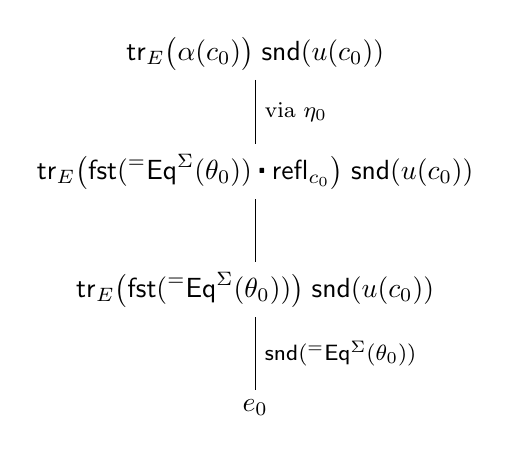
\begin{tikzpicture}
\node (N0) at (0,3) {$\trans_E\big(\alpha(c_0)\big) \; \snd(u(c_0))$};
\node (N1) at (0,1.5) {$\trans_E\big(\fst(\idtodpair(\theta_0)) \ct \refl_{c_0}\big) \; \snd(u(c_0))$};
\node (N2) at (0,0) {$\trans_E\big(\fst(\idtodpair(\theta_0))\big) \; \snd(u(c_0))$};
\node (N3) at (0,-1.5) {$e_0$};
\draw[-] (N0) -- node[right]{\footnotesize via $\eta_0$} (N1);
\draw[-] (N1) -- node[right]{\footnotesize} (N2);
\draw[-] (N2) -- node[right]{\footnotesize $\snd(\idtodpair(\theta_0))$} (N3);
\end{tikzpicture}
\end{center}
and $\phi_1$ is defined analogously.
\end{proof}

\begin{theorem}\label{lem:BoolMainInt}
In $\Hint$, the following conditions on an algebra $\X : \BoolAlg_{\UU_i}$ are equivalent:
\begin{enumerate}
\item $\X$ satisfies the induction principle on the universe $\UU_j$
\item $\X$ satisfies the recursion and recursion uniqueness principles on the universe $\UU_j$
\item $\X$ is homotopy-initial on the universe $\UU_j$  
\end{enumerate}
for $j \geq i$. In other words, we have \[ \HasBoolInd_{\UU_j}(\X)  \;\; \simeq \;\; \HasBoolRec_{\UU_j}(\X) \times \HasBoolRecUniq_{\UU_j}(\X) \;\; \simeq \;\; \IsBoolHInit_{\UU_j}(\X) \]
provided $j \geq i$. Furthermore, all 3 conditions are mere propositions.
\end{theorem}
\begin{proof}
Conditions (1) and (3) are mere propositions by Lem.~\ref{lem:IsContrIsProp} (for the latter), Lem.~\ref{lem:PropChar},~\ref{lem:BoolIndImpUniqInt} (for the former), and the fact that a family of mere propositions is itself a mere proposition.
\end{proof}

Furthermore, we have the following corollary which does \emph{not} have an analogue in the extensional case:
\begin{corollary}\label{BoolHInitIso}
In $\Hint$, any two algebras $\X,\Y : \BoolAlg_{\UU_i}$ which are homotopy-initial on $\UU_i$ are equal:
\[ \IsBoolHInit_{\UU_i}(\X) \to \IsBoolHInit_{\UU_i}(\Y) \to \X = \Y\] 
\end{corollary}
\begin{proof}
By Lem.~\ref{BoolAlgSpace} it suffices to construct an isomorphism between $\X$ and $\Y$. Since $\X$ and $\Y$ are both homotopy-initial on $\UU_i$, there exist homomorphisms $\mu : \BoolHom \; \X \; \Y$ and $\nu : \BoolHom \; \Y \; \X$. Again by homotopy-initiality, we have $\nu \comp \mu = \one_\X$ and $\mu \comp \nu = \one_\Y$, which gives us the desired isomorphism.
\end{proof}

We can thus characterize the type $\Bool$ using the universal property of homotopy-initiality as follows.
\begin{corollary}\label{lem:BoolInitInt}
In $\Hint$ extended with the type $\Bool$, the algebra $(\Bool,0,1) : \BoolAlg_{\UU_0}$ is homotopy-initial on any universe $\UU_j$.
\end{corollary}

\begin{corollary}\label{lem:BoolCharInt}
In $\Hint$ extended with an algebra $\X : \BoolAlg_{\UU_0}$ which is homotopy-initial on any universe $\UU_j$, the type $\Bool$ with propositional computation rules is definable. 
\end{corollary}
\begin{proof}
We have an algebra $\cdot \vdash \X : \BoolAlg_{\UU_0}$ such that for any $j$, there exists a term $\cdot \vdash h_j  : \IsBoolHInit_{\UU_j}(\X)$. Since the requirement $j \geq 0$ always holds, Cor.~\ref{lem:BoolMainInt} implies that for any $j$, we have a term $\cdot \vdash r_j : \HasBoolInd_{\UU_j}(\X)$. This implies that the type $\Bool$ with propositional computation rules is definable.
\end{proof}

Corollaries~\ref{lem:BoolCharInt} and \ref{lem:BoolInitInt} are the analogue in Homotopy Type Theory of the characterization of 
$\Bool$ as a strict coproduct $1+1$ in extensional type theory. It makes precise the rough idea that, 
in intensional type theory, $\Bool$ is a kind of homotopy coproduct or weak $\omega$-coproduct 
in the weak $\omega$-category $\mathcal{C}(\Hint)$ of types, terms, identity terms, higher identity terms, \ldots.  
It is worth emphasizing that homotopy-initiality is a purely type-theoretic notion; despite having an obvious semantic interpretation, it is formulated in terms of inhabitation of specific, definable types. Indeed, Corollary~\ref{lem:BoolMainInt} and its proof have been completely formalized in the Coq proof assistant~\cite{AwodeyS:indtht}.



%%%%%%%%%%%%%%%%%%%%%%%%%%%%%%%%%%%%%%%%%%%%%%%%%%%%%%%%%%%%%%%%%%%%%%%%%%%%%%%%%%%%%%%%%%%%%%%%%%%%%%%%%%
%%%%%%%%%%%%%%%%%%%%%%%%%%%%%%%%%%%%%%%%%%%%%%%%%%%%%%%%%%%%%%%%%%%%%%%%%%%%%%%%%%%%%%%%%%%%%%%%%%%%%%%%%%

\newpage

\section{W-types}
\label{section:wfiles}

\subsection{W-types: extensional case}

We recall the rules for W-types from~\cite{MartinLofP:inttt}; to state them more conveniently, we sometimes write $\W$ instead of $\W^{\UU_i}_{x : A}B(x)$; $\wsup(a,t)$ instead of $\wsup^{A,x.B}_{\UU_i}(a,t)$; and $\wind(m)$ instead of $\wind^{A,x.B}_{\UU_j}\big(w.E,a.t.s.e,m\big)$.

\smallskip

\begin{itemize}
\item $\W$-formation rule.\smallskip
\[
\begin{prooftree}
 A : \UU_i \qquad
 x:A \vdash B(x) : \UU_i
 \justifies
 \W^{\UU_i}_{x : A}B(x)
\end{prooftree}
\]
\item $\W$-introduction rule.\smallskip
\[
\begin{prooftree}
A : \UU_i \qquad
x:A \vdash B(x) : \UU_i \qquad
a:A \qquad
t : B(a) \to \W
\justifies
\wsup^{A,x.B}_{\UU_i}(a,t): \W
\end{prooftree}
\]
\item $\W$-elimination rule.\smallskip
\begin{mathpar}
\inferrule{A : \UU_i \\ x:A \vdash B(x) : \UU_i \\ m : \W \\ w : \W \vdash E(w) : \UU_j \\ x:A, p: B(x) \to \W, r : \prd{b:B(x)} E(p \;b) \vdash e(x,p,r) :E(\wsup(x,p))}{\wind^{A,x.B}_{\UU_j}\big(w.E,x.p.r.e,m\big) : E(m)}
\end{mathpar}
\item $\W$-computation rule.\smallskip
\begin{mathpar}
\inferrule{A : \UU_i \\ x:A \vdash B(x) : \UU_i \\ a : A \\ t : B(a) \to \W \\ w : \W \vdash E(w) : \UU_j \\ x:A, p: B(x) \to \W, r : \prd{b:B(x)} E(p \;b) \vdash
e(x,p,r) :E(\wsup(x,p))}
{\wind(\wsup(a,t)) \equiv e(a,t,\lam{b:B(a)} \wind(t\;b)) : E(\wsup(a,t))}
\end{mathpar}
\end{itemize}

\noindent
\medskip

W-types can be seen informally as the free algebras for signatures
with operations of possibly infinite arity, but no equations. Indeed, the premises 
of the formation rule above can be thought of as specifying a signature that has the elements of~$A$ 
as operations and in which the arity of $a : A$ is the cardinality of the type $B(a)$. Then, the introduction rule specifies the canonical way of forming an element of the free algebra, and the elimination rule can be seen as the propositions-as-types translation of the appropriate induction principle.

As before, the above rules imply a non-dependent version of elimination and the corresponding computation rule, where we write $\wrec(m)$ instead of $\wrec^{A,x.B}_{\UU_j}\big(C,x.r.c,m\big)$ where appropriate. \smallskip
\begin{itemize}
\item Simple $\W$-elimination rule.\smallskip
\begin{mathpar}
\inferrule{A : \UU_i \\ x:A \vdash B(x) : \UU_i \\ m : \W \\ C : \UU_j \\x:A, r : B(x) \to C \vdash c(x,r) : C}{\wrec^{A,x.B}_{\UU_j}\big(C,x.r.c,m\big) : C}
\end{mathpar}
\item Simple $\W$-computation rule.\smallskip
\begin{mathpar}
\inferrule{A : \UU_i \\ x:A \vdash B(x) : \UU_i \\ a : A \\ t : B(a) \to \W \\ C : \UU_j \\ x:A, r : B(x) \to C \vdash c(x,r) : C}
{\wrec(\wsup(a,t)) \equiv c(a,\lam{b:B(a)} \wrec(t \;b)) : C}
\end{mathpar}
\end{itemize} \smallskip

The induction principle also implies the following uniqueness principles, which state that any two functions out of $\W$ which satisfy the same recurrence are pointwise equal:
\begin{itemize}
\item $\W$-uniqueness principle.\smallskip
\begin{mathpar}
\inferrule{A : \UU_i \\ x:A \vdash B(x) : \UU_i \\ m : \W \\ w:\W \vdash E(w) : \UU_j \\ x:A, p: B(x) \to \W, r : \prd{b:B(x)} E(p \;b) \vdash
e(x,p,r) :E(\wsup(x,p)) \\ w:\W \vdash f(w) : E(w) \\ x:A, p: B(x) \to \W \vdash f(\wsup(x,p)) \equiv e(x,p,\lam{b:B(x)} f(p \;b)) \\ w:\W \vdash g(w) : E(w) \\ x:A, p: B(x) \to \W \vdash g(\wsup(x,p)) \equiv e(x,p,\lam{b:B(x)} g(p \;b))}{f(m) \equiv g(m) : E(m)}
\end{mathpar}
\item Simple $\W$-uniqueness principle.\smallskip
\begin{mathpar}
\inferrule{A : \UU_i \\ x:A \vdash B(x) : \UU_i \\ m : \W \\ C : \UU_j \\ x:A, r : B(x) \to C \vdash c(x,r) : C \\ w:\W\vdash f(w) : C \\ x:A, p: B(x) \to \W \vdash f(\wsup(x,p)) \equiv c(x,\lam{b:B(x)} f(p \;b)) \\ w:\W\vdash g(x) : C \\ x:A, p: B(x) \to \W \vdash g(\wsup(x,p)) \equiv c(x,\lam{b:B(x)} g(p \;b))}{f(m) \equiv g(m) : C}
\end{mathpar}
\end{itemize} \smallskip
As before, we can prove the dependent uniqueness principle by using the induction principle with the type family $w \mapsto f(w) =_{E(w)} g(w)$. For this we need to show that for any $x,p$ we have $f(\wsup(x,p)) = g(\wsup(x,p))$ under the induction hypothesis $\prd{b:B(x)} f(p\;b) = g(p\;b)$. Using this hypothesis with function extensionality we get $\lam{b:B(x)} f(p\;b) = \lam{b:B(x)} g(p\;b)$. Together with the premises of the uniqueness rule this gives us $f(\wsup(a,t)) = g(\wsup(a,t))$ as desired. The induction principle thus gives us pointwise propositional equality between $f$ and $g$ and we appeal to the identity reflection rule to finish the proof. The simple uniqueness principle again follows from the dependent one.

We can now formulate the notions of algebras, homomorphisms, etc. accordingly:

\begin{definition}\label{def:WAlg}
For $A:\UU_i$, $B : A \to \UU_i$, define the type of \emph{$\W$-algebras} on a universe $\UU_j$ as
\[\WAlg_{\UU_j}(A,B) \; \defeq \sm{C : \UU_j} \prd{a:A} (B(a) \to C) \to C \]
\end{definition}

\begin{definition}\label{def:WFibAlg}
For $A:\UU_i$, $B : A \to \UU_i$, define the type of \emph{fibered $\W$-algebras} on a universe $\UU_k$ over $\mathcal{X} : \WAlg_{\UU_j}(A,B)$ by
\[\WFibAlg_{\UU_k}(A,B) \; (C,c) \defeq \sm{E : C \to \UU_k} \prd{a:A}\prd{t: B(a) \to C} \big(\prd{b:B(a)} E(t \;b) \big) \to E(c(a,t)) \]
\end{definition}

\begin{definition}\label{def:WHom}
For $A:\UU_i$, $B : A \to \UU_i$, $\X : \WAlg_{\UU_j}(A,B)$, $\Y : \WAlg_{\UU_k}(A,B)$, define the type of \emph{$\W$-homomorphisms} from $\X$ to $\Y$ by
\[ \WHom \; (C,c) \; (D,d) \defeq \sm{f:C\to D}\prd{a:A}\prd{t: B(a) \to C} f(c(a,t)) = d(a,\lam{b:B(a)} f(t\;b)) \]
\end{definition}

\begin{definition}\label{def:WFibHom}
For $A:\UU_i$, $B : A \to \UU_i$, $\X : \WAlg_{\UU_j}(A,B)$, $\Y : \WFibAlg_{\UU_k}(A,B) \; \X$, define the type of \emph{fibered $\W$-homomorphisms} from $\X$ to $\Y$ by
\[ \WFibHom \; (C,c) \; (E,e) \defeq \sm{(f:\prd{x:C}E(x))}\prd{a:A}\prd{t: B(a) \to C} f(c(a,t)) = e(a,t,\lam{b:B(a)} f(t\;b)) \]
\end{definition}

\begin{definition}\label{def:WRec}
For $A:\UU_i$, $B : A \to \UU_i$, an algebra $\X : \WAlg_{\UU_j}(A,B)$ \emph{satisfies the recursion principle} on a universe $\UU_k$ if for any algebra $\Y : \WAlg_{\UU_k}(A,B)$ there exists
a $\W$-homomorphism between $\X$ and $\Y$:
\[ \HasWRec_{\UU_k}(\X) \defeq \prd{(\Y:\WAlg_{\UU_k}(A,B))} \WHom \; \X \; \Y \]
\end{definition}

\begin{definition}\label{def:WInd}
For $A:\UU_i$, $B : A \to \UU_i$, an algebra $\X : \WAlg_{\UU_j}(A,B)$ \emph{satisfies the induction principle} on a universe $\UU_k$ if for any fibered algebra $\Y : \WFibAlg_{\UU_k}(A,B) \; \X$ there exists a fibered $\W$-homomorphism between $\X$ and $\Y$:
\[ \HasWInd_{\UU_k}(\X) \defeq \prd{(\Y:\WFibAlg_{\UU_k}(A,B) \; \X)} \WFibHom \; \X \; \Y \]
\end{definition}

\begin{definition}\label{def:WRecUniq}
For $A:\UU_i$, $B : A \to \UU_i$, an algebra $\X : \WAlg_{\UU_j}(A,B)$ \emph{satisfies the recursion uniqueness principle} on a universe $\UU_k$ if for any algebra $\Y : \WAlg_{\UU_k}(A,B)$
any two $\W$-homomorphisms between $\X$ and $\Y$ are equal:
\[ \HasWRecUniq_{\UU_k}(\X) \defeq \prd{(\Y:\WAlg_{\UU_k}(A,B))} \isprop(\WHom \; \X \; \Y) \]
\end{definition}

\begin{definition}\label{def:WIndUniq}
For $A:\UU_i$ and $B : A \to \UU_i$, an algebra $\X : \WAlg_{\UU_j}(A,B)$ \emph{satisfies the induction uniqueness principle} on a universe $\UU_k$ if for any fibered algebra $\Y : \WFibAlg_{\UU_k}(A,B) \; \X$ any two fibered $\W$-homomorphisms between $\X$ and $\Y$ are equal:
\[ \HasWIndUniq_{\UU_k}(\X) \defeq \prd{(\Y:\WFibAlg_{\UU_k}(A,B) \; \X)} \isprop(\WFibHom \; \X \; \Y) \]
\end{definition}

\begin{definition}\label{def:WInit}
For $A:\UU_i$ and $B : A \to \UU_i$, an algebra $\X : \WAlg_{\UU_j}(A,B)$ is \emph{initial} on a universe $\UU_k$ if for any algebra $\Y : \WAlg_{\UU_k}(A,B)$ there exists a unique $\W$-homomorphism between $\X$ and $\Y$:
\[ \IsWInit_{\UU_k}(\X) \defeq \prd{(\Y:\WAlg_{\UU_k}(A,B))} \iscontr(\WHom \; \X \; \Y) \]  
\end{definition}

As before, the induction principle implies induction uniqueness:

\begin{lemma}\label{lem:WIndImpUniq}
In $\Hext$, for $A:\UU_i$, $B : A \to \UU_i$, if an algebra $\X : \WAlg_{\UU_j}(A,B)$ satisfies the induction principle on the universe $\UU_k$, it also satisfies the induction uniqueness principle on $\UU_k$. In other words, we have
\[ \HasWInd_{\UU_k}(\X) \;\; \rightarrow \;\; \HasWIndUniq_{\UU_k}(\X) \]
\end{lemma}
\begin{proof}
Let an algebra $(C,c) : \WAlg_{\UU_j}(A,B)$ be given. To prove the induction uniqueness principle, take any algebra $(E,e) : \WFibAlg_{\UU_k} \; (C,c)$ and homomorphisms $(f,\gamma), (g,\delta) : \WFibHom \; (C,c) \; (E,e)$. Because of UIP, showing $(f,\gamma) = (g,\delta)$ is equivalent to showing $f = g$. For the latter, we use the induction principle with the fibered algebra $\big(x \mapsto f(x) = g(x); a,t,s \mapsto \refl(f(c(a,t)) \big)$. This is indeed well-typed since $\gamma(a,t)$ gives us $f(c(a,t)) = e(a,t,\lam{b:B(a)} f(t\;b))$; $\delta(a,t)$ gives us $g(c(a,t)) = e(a,t,\lam{b:B(a)} g(t\;b))$; and $s$ together with function extensionality gives us
$\lam{b:B(a)} f(t\;b) = \lam{b:B(a)} g(t\;b)$.

The first component of the resulting homomorphism together with the function extensionality principle then give us $f = g$.
\end{proof}

%\begin{lemma}\label{lem:WRecUniqEqInit}
%In $\Hext$, for $A:\UU_i$, $B : A \to \UU_i$, the following conditions on an algebra $\X : \WAlg_{\UU_j}(A,B)$ are equivalent:
%\begin{enumerate}
%\item $\X$ satisfies the recursion and recursion uniqueness principles on the universe $\UU_k$
%\item $\X$ is initial on the universe $\UU_k$
%\end{enumerate}
%In other words, we have
%\[ \HasWRec_{\UU_k}(\X) \times \HasWRecUniq_{\UU_k}(\X) \;\; \simeq \;\; \IsWInit_{\UU_k}(\X) \]
%\end{lemma}
%\begin{proof}
%By Lem.~\ref{lem:ContrChar}.
%\end{proof}

\begin{corollary}\label{lem:WIndImpInit}
In $\Hext$, for $A:\UU_i$, $B : A \to \UU_i$, if an algebra $\X : \WAlg_{\UU_j}(A,B)$ satisfies the induction principle on the universe $\UU_k$, it is initial on $\UU_k$. In other words, we have
\[ \HasWInd_{\UU_k}(\X) \;\; \rightarrow \;\; \IsWInit_{\UU_k}(\X) \]
\end{corollary}

\begin{lemma}\label{lem:WRecUniqImpInd}
In $\Hext$, for $A:\UU_i$, $B : A \to \UU_i$, if an algebra $\X : \WAlg_{\UU_j}(A,B)$ satisfies the recursion and recursion uniqueness principles on the universe $\UU_k$ and $k \geq j$, then it satisfies the induction principle on $\UU_k$. In other words, we have
\[ \HasWRec_{\UU_k}(\X) \times \HasWRecUniq_{\UU_k}(\X) \;\; \rightarrow \; \; \HasWInd_{\UU_k}(\X) \]
provided $k \geq j$.
\end{lemma}
\begin{proof}
Let algebras $(C,c) : \WAlg_{\UU_j}(A,B)$ and $(E,e) : \WFibAlg_{\UU_k} \; (C,c)$ be given. 
We use the recursion principle with the algebra $(\sm{x:C} E(x); a,s \mapsto d(a,s))$ where
\[ d(a,s) \defeq \Big(c\big(a,\lam{b:B(a)} \fst(s\;b)\big), e\big(a, \lam{b:B(a)} \fst(s\;b), \lam{b:B(a)} \snd(s\;b)\big) \Big) \big) \]
We note that the carrier type belongs to $\UU_k$ as $j \leq k$. This gives us a homomorphism $(u,\theta)$, where $u : C \to \sm{x:C} E(x)$ and $\theta : \prd{a}\prd{t} u(c(a,t)) = d(a,\lam{b:B(a)}u(t\;b))$. We can now form two homomorphisms 
\[\big(\fst \comp u; a,t \mapsto \refl_{c(a,\lam{b:B(a)}u(t\;b))}\big), \big(\idfun{C}; a,t \mapsto \refl_{c(a,t)}\big) : \WHom \; (C,c) \; (C,c)\] The first one type-checks due to $\theta$. The recursion uniqueness principle tells us that these homomorphisms are equal. Thus, $\fst \comp u = \idfun{C}$ and in particular $\fst \comp u \equiv \idfun{C}$. 

We can thus define the desired fibered homomorphism as \[\big(\snd \comp u; a,t \mapsto \refl(e(a,t,\lam{b:B(a)}\snd(u(t\;b))))\big) : \WFibHom \; (C,c) \; (E,e)\]
which type-checks due to $\theta$ and the fact that $\fst \comp u \equiv \idfun{C}$.
\end{proof}

\begin{corollary}\label{lem:WMain}
In $\Hext$, for $A:\UU_i$, $B : A \to \UU_i$, the following conditions on an algebra $\X : \WAlg_{\UU_j}(A,B)$ are equivalent:
\begin{enumerate}
\item $\X$ satisfies the induction principle on the universe $\UU_k$
\item $\X$ satisfies the recursion and recursion uniqueness principles on the universe $\UU_k$
\item $\X$ is initial on the universe $\UU_k$  
\end{enumerate}
for $k \geq j$. In other words, we have \[ \HasWInd_{\UU_k}(\X)  \;\; \simeq \;\; \HasWRec_{\UU_k}(\X) \times \HasWRecUniq_{\UU_k}(\X) \;\; \simeq \;\; \IsWInit_{\UU_k}(\X) \]
provided $k \geq j$. Furthermore, all 3 conditions are mere propositions.
\end{corollary}
\begin{proof}
Conditions (1) and (3) are mere propositions by Lem.~\ref{lem:IsContrIsProp} (for the latter), Lem.~\ref{lem:PropChar},~\ref{lem:BoolIndImpUniq} (for the former), and the fact that a family of mere propositions is itself a mere proposition.
\end{proof}

We can thus characterize $\W$-types using the universal property of initiality as follows.
\begin{corollary}\label{lem:WInit}
In $\Hext$ with $\W$-types, for any $A:\UU_i$, $B : A \to \UU_i$, the algebra \[\Big(\W^{\UU_i}_{x:A}B(x),\lam{a}\lam{t} \wsup_{\UU_i}^{A,x.B(x)}(a,t) \Big) : \WAlg_{\UU_i}(A,B)\] is initial on any universe $\UU_j$.
\end{corollary}

\begin{corollary}\label{lem:WChar}
In $\Hext$ extended with an algebra $\X_{\UU_i}(A,B) : \WAlg_{\UU_i}(A,B)$ for any $\UU_i$, $A : \UU_i$, $B : A \to \UU_i$, which is initial on any universe $\UU_j$, Martin-L{\"o}f's $\W$-types are definable.
\end{corollary}
\begin{proof}
For any $i$, the algebra $A:\UU_i,B:A\to \UU_i \vdash \X_{\UU_i}(A,B) : \WAlg_{\UU_i}(A,B)$ is such that for any $j$, there exists a term $A:\UU_i,B:A\to \UU_i \vdash h^i_j  : \IsWInit_{\UU_j}(\X_{\UU_i}(A,B))$. By Cor.~\ref{lem:BoolMain}, for any $j \geq i$ there is a term $A:\UU_i,B:A\to \UU_i \vdash r^i_j : \HasWInd_{\UU_j}(\X_{\UU_i}(A,B))$. Since universes are cumulative, this implies that such a term $r^i_j$ exists \emph{for any $j$}. This in turn implies that $\W$-types are definable.
\end{proof}

We conclude by the type-theoretic analogue of Lambek's lemma for $\W$-types, which asserts that the structure map of an initial algebra is an equivalence. In $\Hext$ any equivalence is also a type isomorphism, which then gives us the more familiar formulation of Lambek's lemma.

\begin{lemma}\label{lem:ExtLambek}
Over $\Hext$, for $A:\UU_i$, $B : A \to \UU_i$, if an algebra $(C,c) : \WAlg_{\UU_j}(A,B)$ is initial on $\UU_j$ and $j \geq i$, then the map from $\sm{x:A} B(x) \to C$ to $C$ given by $c$ is an equivalence.
\end{lemma}
\begin{proof}
By abuse of notation we refer to both the curried and uncurried versions of the structure map by $c$. Since $(C,c)$ is initial on $\UU_j$, it satisfies the recursion principle on $\UU_j$. We use it with the algebra \[\Big(\sm{x:A} B(x) \to C; a,s \mapsto \big(a,\lam{b:B(a)} c(s\;b)\big)\Big)\]
We note that the carrier type belongs to $\UU_j$ as $i \leq j$. This gives us a homomorphism $(u,\theta)$ where $u : C \to \big(\sm{x:A} B(x) \to C\big)$ and $\theta : \prd{a}\prd{t} u(c(a,t)) = \big(a,\lam{b:B(a)} c(u(t\;b))\big)$.  We can now form two homomorphisms
\[\big(c \comp u; a,t \mapsto \refl_{c(a,\lam{b:B(a)}u(t\;b))}\big), \big(\idfun{C}; a,t \mapsto \refl_{c(a,t)}\big) : \WHom \; (C,c) \; (C,c)\] where the first one type-checks due to $\theta$. Since $(C,c)$ is initial on $\UU_j$, it satisfies the recursion uniqueness principle on $\UU_j$, thus the above homomorphisms are equal. Thus, we have $c \comp u = \idfun{C}$, hence $c \comp u \sim \idfun{C}$ and also $c \comp u \equiv \idfun{C}$. The latter together with $\theta$ implies that for any $a,t$, we have $u(c(a,t)) \equiv (a,t)$. Thus $u \comp c \sim \idfun{\sm{x:A} B(x) \to C}$.
\end{proof}

\begin{corollary}
Over $\Hext$, given $A:\UU_i$, $B : A \to \UU_i$ and $a_1,a_2:A$, $t_1 : B(a_1) \to \W$, $t_2 : B(a_2) \to \W$ we have
\[ \wsup(a_1,t_1) = \wsup(a_2,t_2) \;\;\; \simeq \;\;\; (a_1,t_1) = (a_2,t_2)\]
\end{corollary}
\begin{proof}
By Lem.~\ref{lem:ExtLambek} and Cor.~\ref{lem:WInit}, the structure map $\wsup$ defines an equivalence between $\sm{x:A} B(x) \to \W$ and $\W$. The rest follows from Lem.~\ref{lem:apeq}\ednote{Which says that $a = b$ is equivalent to $f(a) = f(b)$ if $f$ is an equivalence}.
\end{proof}


\subsection{W-types: intensional case}


Although it is more elaborate to state (and difficult to prove) owing to the presence of 
recursively generated data, our main result on  W-types is analogous to 
the foregoing example in the following respect: rather than being strict initial algebras, as in the 
extensional case, W-types with propositional computation rules are instead homotopy-initial algebras. This fact can again be stated 
entirely syntactically, as an equivalence between the definability of W-types with propositional computation rules (which we spell
out below) and the existence of a suitable family of homotopy-initial algebras.  Moreover, as in the simple case of the type $\Bool$ above, the proof is again entirely constructive.

The propositional computation rules for W-types are as follows:\smallskip
\begin{itemize}
\item Propositional $\W$-computation rule.\smallskip
\begin{mathpar}
\inferrule{A : \UU_i \\ x:A \vdash B(x) : \UU_i \\ a : A \\ t : B(a) \to \W \\ w : \W \vdash E(w) : \UU_j \\ x:A, p: B(x) \to \W, r : \prd{b:B(x)} E(p \;b) \vdash e(x,p,r) :E(\wsup(x,p))}
{\windcomp_{\UU_i}(A,x.B,w.E,x.p.r.e,a,t):\wind(\wsup(a,t)) = e(a,t,\lam{b:B(a)} \wind(t\;b))}
\end{mathpar}
\item Simple propositional $\W$-computation rule.\smallskip
\begin{mathpar}
\inferrule{A : \UU_i \\ x:A \vdash B(x) : \UU_i \\ a : A \\ t : B(a) \to \W \\ C : \UU_j \\ x:A, r : B(x) \to C \vdash c(x,r) : C}
{\wreccomp_{\UU_i}(A,x.B,C,x.r.c,a,t) : \wrec(\wsup(a,t)) = c(a,\lam{b:B(a)} \wrec(t \;b))}
\end{mathpar}
\end{itemize}\smallskip

\begin{remark}\label{thm:wtypesinvariance}
One interesting aspect of this group of rules is that, unlike the standard rules for $\W$-types, they are invariant under equivalence, and propositional equality in particular. 
If $A:\UU_i$ and $x:A \vdash B(x):\UU_i$ and we have a type $W : \UU_i$ such that $W \simeq \W^{\UU_i}_{x:A} B(x)$, then $W$ can be shown to satisfy the same rules as $\W^{\UU_i}_{x:A} B(x)$, in the sense that there are definable terms playing the role of the primitive constants that appear in the rules for $\W^{\UU_i}_{x:A} B(x)$.
\end{remark}

We again have uniqueness principles, in the propositional form:
\begin{itemize}
\item Propositional $\W$-uniqueness principle.\smallskip
\begin{mathpar}
\inferrule{A : \UU_i \\ x:A \vdash B(x) : \UU_i \\ m : \W \\ w:\W \vdash E(w) : \UU_j \\ x:A, p: B(x) \to \W, r : \prd{b:B(x)} E(p \;b) \vdash e(x,p,r) :E(\wsup(x,p)) \\ w:\W \vdash f(w) : E(w) \\ w:\W \vdash g(w) : E(w) \\ x:A, p: B(x) \to \W \vdash \gamma(x,p) : f(\wsup(x,p)) = e(x,p,\lam{b:B(x)} f(p \;b)) \\ x:A, p: B(x) \to \W \vdash \delta(x,p) : g(\wsup(x,p)) = e(x,p,\lam{b:B(x)} g(p \;b))}
{\winduniq_{\UU_i}(A,x.B,w.E,x.p.r.e,w.f,x.p.\gamma,w.g,x.p.\delta,m) : f(m) = g(m)}
\end{mathpar}
\item Simple propositional $\W$-uniqueness principle.\smallskip
\begin{mathpar}
\inferrule{A : \UU_i \\ x:A \vdash B(x) : \UU_i \\ m : \W \\ C : \UU_j \\ x:A, r : B(x) \to C \vdash c(x,r) : C \\ w:\W\vdash f(w) : C \\ x:A, p: B(x) \to \W \vdash \gamma(x,p) : f(\wsup(x,p)) = c(x,\lam{b:B(x)} f(p \;b)) \\ w:\W\vdash g(x) : C \\ x:A, p: B(x) \to \W \vdash \delta(x,p) : g(\wsup(x,p)) = c(x,\lam{b:B(x)} g(p \;b))}
{\wrecuniq_{\UU_i}(A,x.B,C,x.r.c,w.f,x.p.\gamma,w.g,x.p.\delta,m) : f(m) = g(m)}
\end{mathpar}
\end{itemize} \smallskip
The witness terms will be shortened to $\winduniq(m), \wrecuniq(m)$ where appropriate. In showing the above laws, we proceed analogously to the extensional case: we use the induction principle with the type family $x \mapsto f(w) =_{E(w)} g(w)$. For this we need to show that for any $x,p$ we have $f(\wsup(x,p)) = g(\wsup(x,p))$ under the induction hypothesis $h : \prd{b:B(x)} f(p\;b) = g(p\;b)$. We can construct this path explicitly as 
\[ \gamma(x,p) \ct \app_{e(x,p,-)}(\funext(h))\ct \delta(x,p)^{-1} \]
The simple uniqueness rule again follows from the dependent one. Invoking the corresponding (propositional) computation rule, we  get the following coherence principles for W-types:
\begin{itemize}
\item Propositional $\W$-coherence principle.\smallskip
\begin{mathpar}
\inferrule{A : \UU_i \\ x:A \vdash B(x) : \UU_i \\ a : A \\ t : B(a) \to \W \\ w:\W \vdash E(w) : \UU_j \\ x:A, p: B(x) \to \W, r : \prd{b:B(x)} E(p \;b) \vdash e(x,p,r) :E(\wsup(x,p)) \\ w:\W \vdash f(w) : E(w) \\ w:\W \vdash g(w) : E(w) \\ x:A, p: B(x) \to \W \vdash \gamma(x,p) : f(\wsup(x,p)) = e(x,p,\lam{b:B(x)} f(p \;b)) \\ x:A, p: B(x) \to \W \vdash \delta(x,p) : g(\wsup(x,p)) = e(x,p,\lam{b:B(x)} g(p \;b))}
{\windcoh_{\UU_i}(A,x.B,w.E,x.p.r.e,w.f,x.p.\gamma,w.g,x.p.\delta,a,t) : \\ \winduniq(\wsup(a,t)) = \gamma(a,t) \ct \app_{e(a,t,-)}(\funext(\lam{b:B(a)}\winduniq(t\;b)))\ct \delta(a,t)^{-1}}
\end{mathpar}
\item Simple propositional $\W$-coherence principle.\smallskip
\begin{mathpar}
\inferrule{A : \UU_i \\ x:A \vdash B(x) : \UU_i \\ a : A \\ t : B(a) \to \W \\ C : \UU_j \\ x:A, r : B(x) \to C \vdash c(x,r) : C \\ w:\W\vdash f(w) : C \\ x:A, p: B(x) \to \W \vdash \gamma(x,p) : f(\wsup(x,p)) = c(x,\lam{b:B(x)} f(p \;b)) \\ w:\W\vdash g(x) : C \\ x:A, p: B(x) \to \W \vdash \delta(x,p) : g(\wsup(x,p)) = c(x,\lam{b:B(x)} g(p \;b))}
{\wreccoh_{\UU_i}(A,x.B,C,x.r.c,w.f,x.p.\gamma,w.g,x.p.\delta,a,t) : \\ \wrecuniq(\wsup(a,t)) = \gamma(a,t) \ct \app_{c(a,-)}(\funext(\lam{b:B(a)}\wrecuniq(t\;b)))\ct \delta(a,t)^{-1}}
\end{mathpar}
\end{itemize} \smallskip
This motivates the following definitions:

\begin{definition}\label{def:WCell}
For $A:\UU_i$, $B : A \to \UU_i$, $\X : \WAlg_{\UU_j}(A,B)$, $\Y : \WAlg_{\UU_k}(A,B)$ and homomorphisms $\mu, \nu : \WHom \; \X \; \Y$, define the type of \emph{2-cells} between $\mu$ and $\nu$ by
\begin{align*} & \WCell \; (C,c) \; (D,d) \; (f,\gamma) \; (g,\delta) \defeq \\ & \;\;\; \;\;\;\WFibHom \; (C,c) \; \Big(f \sim g; x,p,r \mapsto \gamma(x,p) \ct \app_{d(x)}(\funext(r)) \ct \delta(x,p)^{-1}\Big)
\end{align*}
\end{definition}

\begin{definition}\label{def:WFibCell}
For $A:\UU_i$, $B : A \to \UU_i$, $\X : \WAlg_{\UU_j}(A,B)$, $\Y : \WFibAlg_{\UU_k}(A,B) \; \X$ and fibered homomorphisms $\mu, \nu : \WFibHom \; \X \; \Y$, define the type of \emph{fibered 2-cells} between $\mu$ and $\nu$ by
\begin{align*} & \WFibCell \; (C,c) \; (E, e) \; (f,\gamma) \; (g,\delta) \defeq \\ & \;\;\; \;\;\;\WFibHom \; (C,c) \; \Big(f \sim g; x,p,r \mapsto \gamma(x,p) \ct \app_{e(x,p)}(\funext(r)) \ct \delta(x,p)^{-1}\Big)
\end{align*}
\end{definition}
For brevity, we will often leave out the first two arguments. As expected, we have:
\begin{definition}\label{def:WHInit}
Given $A:\UU_i$, $B : A \to \UU_i$, an algebra $\X : \WAlg_{\UU_j}(A,B)$ is called \emph{homotopy-initial} on a universe $\UU_k$ if for any algebra $\Y : \WAlg_{\UU_k}(A,B)$, the type of $\W$-homomorphisms between $\X$ and $\Y$ is contractible:
\[ \IsWHInit_{\UU_k}(\X) \defeq \prd{(\Y:\WAlg_{\UU_k}(A,B))} \iscontr(\WHom \; \X \; \Y) \]  
\end{definition}

\begin{definition}
For $A:\UU_i$, $B : A \to \UU_i$, $\X : \WAlg_{\UU_j}(A,B)$ there is a designated \emph{identity} homomorphism from $\X$ to itself, defined by
\[ \WIdHom \; (C,c) \defeq (\idfun{C}; a,t \mapsto \refl_{c(a,t)}) \]
\end{definition}
As before, we denote this homomorphism by $\one_\X$.

\begin{definition}
For $A:\UU_i$, $B : A \to \UU_i$, $\X : \WAlg_{\UU_j}(A,B)$, $\Y : \WAlg_{\UU_k}(A,B)$, $\Z : \WAlg_{\UU_l}(A,B)$ and homomorphisms $\mu : \WHom \; \X \; \Y$, $\nu : \WHom \; \Y \; \Z$, the \emph{composition} of $\mu$ and $\nu$ is a homomorphism from $\X$ to $\Z$ defined by
\begin{align*} & \WCompHom \; (C,c) \; (D,d) \; (E,e) \; (f,\gamma) \; (g,\delta) \defeq  \Big(g \comp f; a,t \mapsto \app_g(\gamma(a,t)) \ct \delta(a, f \comp t) \Big)
\end{align*}
\end{definition}
As before, we often leave out the first three arguments and denote the composition by $\nu \comp \mu$.

\begin{definition}
For $A:\UU_i$, $B : A \to \UU_i$, $\X : \WAlg_{\UU_j}(A,B)$, $\Y : \WAlg_{\UU_k}(A,B)$ we define the type of \emph{isomorphisms} between $\X$ and $\Y$ as
\[\WAlgIso \; \X \; \Y \defeq \sm{(\rho : \WHom \; \X \; \Y)} \Big(\sm{(\mu : \WHom \; \Y \; \X)} \mu \comp \rho = \one_\X \Big) \times \Big(\sm{(\nu : \WHom \; \Y \; \X)} \rho \comp \nu = \one_\Y \Big) \] 
\end{definition}

\begin{lemma}\label{WFibHomSpace}
For $A:\UU_i$, $B : A \to \UU_i$, $\X : \WAlg_{\UU_j}(A,B)$, $\Y : \WFibAlg_{\UU_k}(A,B) \; \X$ and $\mu,\nu : \WFibHom \; \X \; \Y$, the path space $\mu = \nu$ is equivalent to the space of fibered 2-cells between $\mu$ and $\nu$:
\[ \mu = \nu \;\; \simeq \;\; \WFibCell \; \mu \; \nu \] 
\end{lemma}
\begin{proof}
Let algebras $(C,c) : \WAlg_{\UU_j}(A,B)$, $(E,e) : \WFibAlg_{\UU_k}(A,B) \; (C,c)$ and homomorphisms $(f,\gamma), (g,\delta) : \WFibHom \; (C,c) \; (E,e)$ be given. We have
\begin{alignat*}{4}
& (f,\gamma) = (g,\delta) & \simeq \\
& \sm{\alpha : f = g} \Big(\delta = \trans_{\big(h \mapsto \prd{a}\prd{t} h(c(a,t)) = e(a,t,\lam{b} h(t\;b))\big)}(\alpha) \; \gamma\Big) & \simeq \\
& \sm{\alpha : f = g} \Big(\delta = \lam{a} \lam{t} \happly(\alpha,c(a,t))^{-1} \ct \gamma(a,t) \ct \app_{e(a,t)}(\funext (\lam{b}\happly(\alpha,t \; b))) \Big) & \;\;\; \simeq \\
& \sm{\alpha : f \sim g} \Big(\delta = \lam{a} \lam{t} \; \alpha(c(a,t))^{-1} \ct \gamma(a,t) \ct \app_{e(a,t)}(\funext (\lam{b}\; \alpha(t \; b))) \Big) & \simeq \\
& \sm{\alpha : f \sim g} \prd{a}\prd{t}\Big(\delta(a,t) = \alpha(c(a,t))^{-1} \ct \gamma(a,t) \ct \app_{e(a,t)}(\funext (\lam{b}\; \alpha(t \; b))) \Big) & \simeq \\ 
& \sm{\alpha : f \sim g} \prd{a}\prd{t}\Big(\alpha(c(a,t)) = \gamma(a,t) \ct \app_{e(a,t)}(\funext (\lam{b}\; \alpha(t \; b))) \ct \delta(a,t)^{-1} \Big) & \equiv \\ 
& \WFibCell \; (f,\gamma) \; (g,\delta)
\end{alignat*}
\end{proof}

\begin{corollary}\label{WHomSpace}
For $A:\UU_i$, $B : A \to \UU_i$, $\X : \WAlg_{\UU_j}(A,B)$, $\Y : \WAlg_{\UU_k}(A,B)$ and $\mu,\nu : \WHom \; \X \; \Y$, the path space $\mu = \nu$ is equivalent to the space of 2-cells between $\mu$ and $\nu$:
\[ \mu = \nu \;\; \simeq \;\; \WCell \; \mu \; \nu \] 
\end{corollary}

\begin{lemma}\label{WAlgSpace}
Given $A:\UU_i$, $B : A \to \UU_i$ and $\X,\Y : \WAlg_{\UU_j}(A,B)$, the path space $\X = \Y$ is equivalent to the space of isomorphisms between $\X$ and $\Y$:
\[ \X = \Y \;\; \simeq \;\; \WAlgIso \; \X \; \Y \] 
\end{lemma}
\begin{proof}
Let algebras $(C,c), (D,d) : \WAlg_{\UU_j}(A,B)$ be given. We have
\begin{alignat*}{4}
& \WAlgIso \; (C,c) \; (D,d) & \equiv \\
& \sm{\rho : \big(\sm{f:C\to D} \prd{a}\prd{t} f(c(a,t)) = d(a,f \comp t) \big)} \Big(\sm{\mu : \big(\sm{g:D\to C} \prd{a}\prd{s} g(d(a,s)) = c(a,g \comp s)\big)} \mu \comp \rho = \one_{(C,c)} \Big)\; \times & \\
& \;\;\;\;\;\;\;\;\;\;\;\;\;\;\;\;\;\;\;\;\;\;\;\;\;\;\;\;\;\;\;\;\;\;\;\;\;\;\;\;\;\;\;\;\;\;\;\;\;\;\Big(\sm{\nu : \big(\sm{h:D\to C} \prd{a}\prd{s} h(d(a,s))=c(a,h\comp s)\big)} \rho \comp \nu = \one_{(D,d)}\Big) & \;\;\;\;\;\;\; \simeq \\
& \sm{f : C\to D} \sm{\epsilon : (\prd{a}\prd{t} f(c(a,t)) = d(a,f \comp t))} \Big(\sm{g:D\to C} \sm{\gamma : (\prd{a}\prd{s} g(d(a,s)) = c(a,g \comp s))} P_{f,\epsilon,g,\gamma}\Big) \; \times & \\
& \;\;\;\;\;\;\;\;\;\;\;\;\;\;\;\;\;\;\;\;\;\;\;\;\;\;\;\;\;\;\;\;\;\;\;\;\;\;\;\;\;\;\;\;\;\;\;\;\;\; \Big(\sm{h:D\to C} \sm{\delta : (\prd{a}\prd{s} h(d(a,s))=c(a,h\comp s))} Q_{f,\epsilon,h,\delta} \Big) &
\end{alignat*}
where
\begin{align*}
& P_{f,\epsilon,g,\gamma} \defeq \Big(g \comp f; a,t \mapsto \app_g(\epsilon(a,t)) \ct \gamma(a, f \comp t)\Big) = \Big(\idfun{C}; a,t \mapsto \refl_{c(a,t)}\Big) \\
& Q_{f,\epsilon,h,\delta} \defeq \Big(f \comp h; a,s \mapsto \app_f(\delta(a,s)) \ct \epsilon(a, h \comp t)\Big) = \Big(\idfun{D}; a,s \mapsto \refl_{d(a,s)}\Big)
\end{align*}
Now we have
\begin{alignat*}{4}
& P_{f,\epsilon,g,\gamma} & \equiv \\
& \Big(g \comp f; a,t \mapsto \app_g(\epsilon(a,t)) \ct \gamma(a, f \comp t)\Big) = \Big(\idfun{C}; a,t \mapsto \refl_{c(a,t)}\Big) & \simeq \\
& \sm{\alpha : g \comp f = \idfun{C}} \Big(\lam{a}\lam{t} \app_g(\epsilon(a,t)) \ct \gamma(a, f \comp t)\Big) = \trans^{-1}_{\big(i \mapsto \prd{a}\prd{t} i(c(a,t)) = c(a,i \comp t)\big)}(\alpha) \; \Big(\lam{a}\lam{t} \refl_{c(a,t)}\Big) & \;\;\; \simeq \\
& \sm{\alpha : g \comp f = \idfun{C}} \Big(\lam{a}\lam{t} \app_g(\epsilon(a,t)) \ct \gamma(a, f \comp t)\Big) = \lam{a}\lam{t} & \\ & \;\;\;\;\;\;\; \happly(\alpha, c(a,t)) \ct \refl_{c(a,t)} \ct \Big(\app_{c(a)}(\funext(\lam{b} \happly(\alpha, t\;b)))\Big)^{-1} & \;\;\; \simeq \\
& \sm{\alpha : g \comp f = \idfun{C}} \prd{a}\prd{t} \Big(\app_g(\epsilon(a,t)) \ct \gamma(a, f \comp t)\Big) = & \\
& \;\;\;\;\;\;\; \happly(\alpha, c(a,t)) \ct \refl_{c(a,t)} \ct \Big(\app_{c(a)}(\funext(\lam{b} \happly(\alpha, t\;b)))\Big)^{-1} & \;\;\; \simeq \\
& \sm{\alpha : g \comp f \sim \idfun{C}} \prd{a}\prd{t} \Big(\app_g(\epsilon(a,t)) \ct \gamma(a, f \comp t)\Big) = & \\
& \;\;\;\;\;\;\; \alpha(c(a,t)) \ct \refl_{c(a,t)} \ct \Big(\app_{c(a)}(\funext(\lam{b} \; \alpha(t\;b)))\Big)^{-1} & \;\;\; \simeq \\
& \sm{\alpha : g \comp f \sim \idfun{C}} \prd{a}\prd{t} \Big(\alpha(c(a,t)) = \app_g(\epsilon(a,t)) \ct \gamma(a, f \comp t) \ct \app_{c(a)}(\funext(\lam{b} \; \alpha(t\;b)))\Big) &
\end{alignat*}
and analogously
\begin{alignat*}{4}
Q_{f,\epsilon,h,\delta} \simeq \sm{\beta : f \comp h \sim \idfun{D}} \prd{a}\prd{s} \Big(\beta(d(a,s)) = \app_f(\delta(a,s)) \ct \epsilon(a, h \comp s) \ct \app_{d(a)}(\funext(\lam{b} \; \beta(s\;b)))\Big) &
\end{alignat*}
Thus we can express $\WAlgIso \; (C,c) \; (D,d)$ equivalently as the type
\begin{alignat*}{4}
& \sm{f : C\to D} \sm{\epsilon : (\prd{a}\prd{t} f(c(a,t)) = d(a,f \comp t))} \sm{g:D\to C} \sm{\alpha : g \comp f \sim \idfun{C}} \sm{h:D \to C} \sm{\beta : f \comp h \sim \idfun{D}} R_{f,\epsilon,g,\alpha} \times S_{f,\epsilon,h,\beta}
\end{alignat*}
where
\begin{alignat*}{4}
& R_{f,\epsilon,g,\alpha} \defeq \sm{\gamma : (\prd{a}\prd{s} g(d(a,s)) = c(a,g \comp s))} \prd{a}\prd{t} \\ & \;\;\;\;\;\;\;\;\;\;\;\; \alpha(c(a,t)) = \app_g(\epsilon(a,t)) \ct \gamma(a, f \comp t) \ct \app_{c(a)}(\funext(\lam{b} \; \alpha(t\;b))) \\
& S_{f,\epsilon,h,\beta} \defeq \sm{\delta : (\prd{a}\prd{s} h(d(a,s)) = c(a,h \comp s))} \prd{a}\prd{s} \\ & \;\;\;\;\;\;\;\;\;\;\;\; \beta(d(a,s)) = \app_f(\delta(a,s)) \ct \epsilon(a, h \comp s) \ct \app_{d(a)}(\funext(\lam{b} \; \beta(s\;b)))
\end{alignat*}
Now we have
\begin{alignat*}{4}
& S_{f,\epsilon,h,\beta} & \equiv \\
& \sm{\delta : (\prd{a}\prd{s} h(d(a,s)) = c(a,h \comp s))} \prd{a}\prd{s} & \\
& \;\;\;\;\;\;\;\;\;\; \beta(d(a,s)) = \app_f(\delta(a,s)) \ct \epsilon(a, h \comp s) \ct \app_{d(a)}(\funext(\lam{b} \; \beta(s\;b))) & \;\;\; \simeq \\
& \prd{a}\prd{s}\sm{\delta : h(d(a,s)) = c(a,h \comp s)}  & \\
& \;\;\;\;\;\;\;\;\;\; \beta(d(a,s)) = \app_f(\delta) \ct \epsilon(a, h \comp s) \ct \app_{d(a)}(\funext(\lam{b} \; \beta(s\;b))) & \;\;\; \simeq \\
& \prd{a}\prd{s}\sm{\delta : h(d(a,s)) = c(a,h \comp s)}  & \\
& \;\;\;\;\;\;\;\;\;\; \app_f(\delta) = \beta(d(a,s)) \ct \Big(\app_{d(a)}(\funext(\lam{b} \; \beta(s\;b)))\Big)^{-1} \ct \epsilon(a, h \comp s)^{-1} & \;\;\; \simeq \\
& \prd{a}\prd{s}\one & \;\;\; \simeq \\
& \one
\end{alignat*}
by Lem.~\ref{lem_singl_equiv_contr},~\ref{lem_ap_equiv}, and the fact that $g,\alpha,h,\beta$ make $f$ into an equivalence. This last fact also implies that the mapping $t \mapsto f \comp t$ is an equivalence between $B(a) \to C$ and $B(a) \to D$ by Lem.~\ref{lem_equiv_comp}\ednote{Which says that if $f:B \to C$ is an equivalence, then so is the mapping $h \mapsto f \comp h$ between $A \to B$ and $A \to C$}. Thus the mapping $\gamma \mapsto \lam{a}\lam{t} \gamma(a,f \comp t)$ is an equivalence between the types $\prd{a:A}\prd{s:B(a)\to D} g(d(a,s)) = c(a,g \comp s)$ and $\prd{a:A}\prd{t:B(a)\to C} g(d(a,f \comp t)) = c(a,g \comp f \comp t)$. Thus:
\begin{alignat*}{4}
& R_{f,\epsilon,g,\alpha} & \equiv \\
& \sm{\gamma : \big(\prd{a}\prd{s} g(d(a,s)) = c(a,g \comp s)\big)} \prd{a}\prd{t} & \\ 
& \;\;\;\;\;\;\;\;\;\; \alpha(c(a,t)) = \app_g(\epsilon(a,t)) \ct \gamma(a, f \comp t) \ct \app_{c(a)}(\funext(\lam{b} \; \alpha(t\;b))) & \;\;\; \simeq \\
& \sm{\gamma : \big(\prd{a}\prd{t} g(d(a,f \comp t)) = c(a,g \comp f \comp t)\big)} \prd{a}\prd{t} & \\ 
& \;\;\;\;\;\;\;\;\;\; \alpha(c(a,t)) = \app_g(\epsilon(a,t)) \ct \gamma(a,t) \ct \app_{c(a)}(\funext(\lam{b} \; \alpha(t\;b))) & \;\;\; \simeq \\
& \prd{a}\prd{t} \sm{\gamma : g(d(a,f \comp t)) = c(a,g \comp f \comp t)} & \\ 
& \;\;\;\;\;\;\;\;\;\; \alpha(c(a,t)) = \app_g(\epsilon(a,t)) \ct \gamma \ct \app_{c(a)}(\funext(\lam{b} \; \alpha(t\;b))) & \;\;\; \simeq \\
& \prd{a}\prd{t} \sm{\gamma : g(d(a,f \comp t)) = c(a,g \comp f \comp t)} & \\ 
& \;\;\;\;\;\;\;\;\;\; \gamma = \Big(\app_g(\epsilon(a,t))\Big)^{-1} \ct \alpha(c(a,t)) \ct \Big(\app_{c(a)}(\funext(\lam{b} \; \alpha(t\;b)))\Big)^{-1} & \;\;\; \simeq \\
& \prd{a}\prd{t}\one & \;\;\; \simeq \\
& \one
\end{alignat*}
by Lem.~\ref{lem_singl_contr}. Thus, we have
\begin{alignat*}{4}
& \WAlgIso \; (C,c) \; (D,d) & \simeq \\
& \sm{f : C\to D} \sm{g:D\to C} \sm{\alpha : g \comp f \sim \idfun{C}} \sm{h:D \to C} \sm{\beta : f \comp h \sim \idfun{D}} \prd{a}\prd{t} f(c(a,t)) = d(a,f \comp t) & \;\;\; \simeq \\
& \sm{f : C\to D} \isequiv(f) \times \prd{a}\prd{t} f(c(a,t)) = d(a,f \comp t) & \;\;\; \simeq \\
& \sm{p : C \simeq D} \prd{a}\prd{t} \big(\fst(p) \; c(a,t)\big) = d(a, \fst(p) \comp t) & \;\;\; \simeq \\
& \sm{p : C = D} \prd{a}\prd{t} \Big(\fst(\idtoeq(p)) \; c(a,t)\Big) = d\Big(a, \fst(\idtoeq(p)) \comp t\Big) & \;\;\; \equiv \\
& \sm{p : C = D} \prd{a} \prd{t} \Big(\trans_{X \mapsto X}(p) \; c(a,t) = d\Big(a,\fst(\idtoeq(p)) \comp t\Big)\Big) & \simeq \\
& \sm{p : C = D} \prd{a} \prd{t} \Big(c(a,t) = \trans^{-1}_{X \mapsto X}(p) \; d\Big(a,\fst(\idtoeq(p)) \comp t\Big)\Big) & \simeq \\
& \sm{p : C = D} \Big(c = \lam{a}\lam{t}\trans^{-1}_{X \mapsto X}(p) \; d\Big(a,\fst(\idtoeq(p)) \comp t\Big)\Big) & \simeq \\ 
& \sm{p : C = D} \Big(c = \trans^{-1}_{\big(X \mapsto \prd{a:A} (B(a) \to X) \to X\big)}(p) \; d\Big) & \simeq \\ 
& (C,c) = (D,d)
\end{alignat*}
\end{proof}

As desired, the analogues of the lemmas from section \ref{subsection:wtypes} still hold in the setting of homotopy type theory:

\begin{lemma}\label{lem:WIndImpUniqInt}
In $\Hint$, for $A:\UU_i$, $B : A \to \UU_i$, if an algebra $\X : \WAlg_{\UU_j}(A,B)$ satisfies the induction principle on the universe $\UU_k$, it also satisfies the induction uniqueness principle on $\UU_k$. In other words, we have
\[ \HasWInd_{\UU_k}(\X) \;\; \rightarrow \;\; \HasWIndUniq_{\UU_k}(\X) \]
\end{lemma}
\begin{proof}
Let an algebra $(C,c) : \WAlg_{\UU_j}(A,B)$ be given. To prove the induction uniqueness principle, take any algebra $(E,e) : \WFibAlg_{\UU_k}(A,B) \; (C,c)$ and homomorphisms $(f,\gamma), (g,\delta) : \WFibHom \; (C,c) \; (E,e)$. By Lem.~\ref{WFibHomSpace}, to show $(f,\gamma) = (g,\delta)$ it suffices to exhibit a fibered 2-cell between $(f,\gamma)$ and $(g,\delta)$. For this we use the induction principle with the fibered algebra $\Big(f \sim g; x,p,r \mapsto \gamma(x,p) \ct \app_{e(x,p)}(\funext(r)) \ct \delta(x,p)^{-1}\Big)$ and we are done.
\end{proof}

%\begin{lemma}\label{lem:WRecUniqEqInitInt}
%In $\Hint$, for $A:\UU_i$, $B : A \to \UU_i$ the following conditions on an algebra $\X : \WAlg_{\UU_j}(A,B)$ are equivalent:
%\begin{enumerate}
%\item $\X$ satisfies the recursion and recursion uniqueness principles on the universe $\UU_k$
%\item $\X$ is homotopy-initial on the universe $\UU_k$
%\end{enumerate}
%In other words, we have
%\[ \HasWRec_{\UU_k}(\X) \times \HasWRecUniq_{\UU_k}(\X) \;\; \simeq \;\; \IsWHInit_{\UU_k}(\X) \]
%\end{lemma}
%\begin{proof}
%By Lem.~\ref{lem:ContrChar}.
%\end{proof}

\begin{corollary}\label{lem:WIndImpHInitInt}
In $\Hint$, for $A:\UU_i$, $B : A \to \UU_i$, if an algebra $\X : \WAlg_{\UU_j}(A,B)$ satisfies the induction principle on the universe $\UU_k$, it is homotopy-initial on $\UU_k$. In other words, we have
\[ \HasWInd_{\UU_k}(\X) \;\; \rightarrow \;\; \IsWHInit_{\UU_k}(\X) \]
\end{corollary}

\begin{lemma}\label{lem:WRecUniqImpIndInt}
In $\Hint$, for $A:\UU_i$, $B : A \to \UU_i$, if an algebra $\X : \WAlg_{\UU_j}(A,B)$ satisfies the recursion and recursion uniqueness principles on the universe $\UU_k$ and $k \geq j$, then it satisfies the induction principle on $\UU_k$. In other words, we have
\[ \HasWRec_{\UU_k}(\X) \times \HasWRecUniq_{\UU_k}(\X) \;\; \rightarrow \; \; \HasWInd_{\UU_k}(\X) \]
provided $k \geq j$.
\end{lemma}
\begin{proof}
Let algebras $(C,c) : \WAlg_{\UU_j}(A,B)$ and $(E,e) : \WFibAlg_{\UU_k} \; (C,c)$ be given. We use the recursion principle with the algebra $(\sm{x:C} E(x); a,s \mapsto d(a,s))$ where
\[ d(a,s) \defeq \Big(c\big(a,\lam{b:B(a)} \fst(s\;b)\big), e\big(a, \lam{b:B(a)} \fst(s\;b), \lam{b:B(a)} \snd(s\;b)\big) \Big) \]
We note that the carrier type belongs to $\UU_k$ as $j \leq k$. This gives us a homomorphism $(u,\theta)$, where $u : C \to \sm{x:C} E(x)$ and $\theta : \prd{a:A}\prd{t:B(a)\to C} u(c(a,t)) = d(a,\lam{b:B(a)}u(t\;b))$. We can now form two homomorphisms 
\[\Big(\fst \comp u; a,t \mapsto \fst(\idtodpair(\theta(a,t)))\Big), \Big(\idfun{C}; a,t \mapsto \refl_{c(a,t)}\Big) : \WHom \; (C,c) \; (C,c)\]
The recursion uniqueness principle tells us that these homomorphisms are equal. By Cor.~\ref{WHomSpace} this means there exists a 2-cell $(\alpha,\eta)$ between them, i.e., we have 
\begin{align*}
& \alpha : \fst \comp u \sim \idfun{C} \\
& \eta : \prd{a:A}\prd{t:B(a)\to C} \Big(\alpha(c(a,t)) = \fst(\idtodpair(\theta(a,t))) \ct \app_{c(a)}\big(\funext(\lam{b:B(a)} \alpha(t\;b))\big) \ct \refl_{c(a,t)}\Big)
\end{align*}
Now it is easy to see that for any $a : A$, path $p : t_1 =_{B(a) \to C} t_2$, and $s : \prd{b:B(a)} E(t_1 \; b)$, we have a higher path
\[ \epsilon(a,p,s) : \trans_E\big(\app_{c(a)}(p)\big) \; e(a,t_1,s) = e\Big(a,t_2,\big(\lam{b:B(a)} \trans_E(\happly(p,b)) \; (s \; b)\big)\Big) \] 
To show this, we simply use path induction on $p$.

We can thus define the desired fibered homomorphism as \[\Big(x \mapsto \trans_E(\alpha(x)) \; \snd(u(x)); a,t \mapsto \phi(a,t) \Big) : \WFibHom \; (C,c) \; (E,e)\]
where $\phi(a,t)$ is the path
\begin{center}
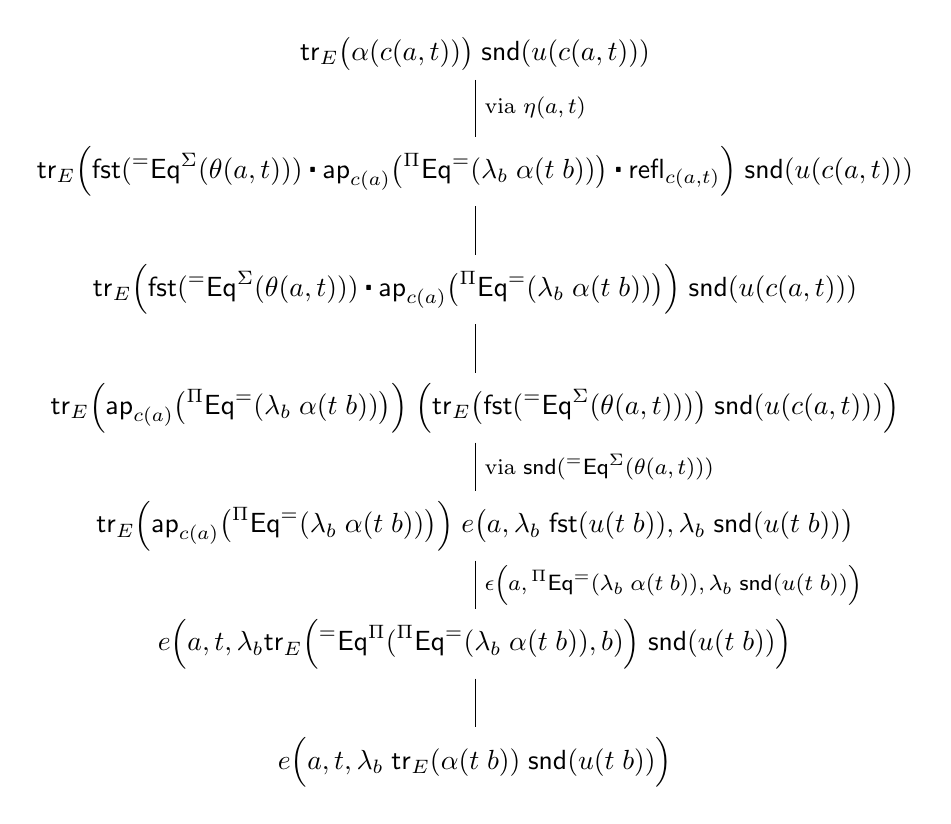
\begin{tikzpicture}
\node (N0) at (0,12) {$\trans_E\big(\alpha(c(a,t))\big) \; \snd(u(c(a,t)))$};
\node (N1) at (0,10.5) {$\trans_E\Big(\fst(\idtodpair(\theta(a,t))) \ct \app_{c(a)}\big(\funext(\lam{b}\; \alpha(t\;b))\big) \ct \refl_{c(a,t)}\Big) \; \snd(u(c(a,t)))$};
\node (N2) at (0,9) {$\trans_E\Big(\fst(\idtodpair(\theta(a,t))) \ct \app_{c(a)}\big(\funext(\lam{b} \;\alpha(t\;b))\big)\Big) \; \snd(u(c(a,t)))$};
\node (N3) at (0,7.5) {$\trans_E\Big(\app_{c(a)}\big(\funext(\lam{b} \; \alpha(t\;b))\big)\Big) \; \Big(\trans_E\big(\fst(\idtodpair(\theta(a,t)))\big) \; \snd(u(c(a,t)))\Big)$};
\node (N4) at (0,6) {$\trans_E\Big(\app_{c(a)}\big(\funext(\lam{b}\; \alpha(t\;b))\big)\Big) \; e\big(a, \lam{b} \;\fst(u(t\;b)), \lam{b}\; \snd(u(t\;b))\big) $};
\node (N5) at (0,4.5) {$e\Big(a,t,\lam{b} \trans_E\Big(\happly(\funext(\lam{b}\; \alpha(t\;b)),b)\Big) \; \snd(u(t\;b))\Big)$};
\node (N6) at (0,3) {$e\Big(a,t,\lam{b} \; \trans_E(\alpha(t\;b)) \; \snd(u(t\;b))\Big)$};

\draw[-] (N0) -- node[right]{\footnotesize via $\eta(a,t)$} (N1);
\draw[-] (N1) -- node[right]{\footnotesize} (N2);
\draw[-] (N2) -- node[right]{\footnotesize} (N3);
\draw[-] (N3) -- node[right]{\footnotesize via $\snd(\idtodpair(\theta(a,t)))$} (N4);
\draw[-] (N4) -- node[right]{\footnotesize $\epsilon\Big(a,\funext(\lam{b} \; \alpha(t\;b)), \lam{b} \; \snd(u(t\;b))\Big)$} (N5);
\draw[-] (N5) -- node[right]{\footnotesize} (N6);
\end{tikzpicture}
\end{center}
\end{proof}

\begin{corollary}\label{lem:WMainInt}
In $\Hint$, for $A:\UU_i$, $B : A \to \UU_i$, the following conditions on an algebra $\X : \WAlg_{\UU_j}(A,B)$ are equivalent:
\begin{enumerate}
\item $\X$ satisfies the induction principle on the universe $\UU_k$
\item $\X$ satisfies the recursion and recursion uniqueness principles on the universe $\UU_k$
\item $\X$ is homotopy-initial on the universe $\UU_k$  
\end{enumerate}
for $k \geq j$. In other words, we have \[ \HasWInd_{\UU_k}(\X)  \;\; \simeq \;\; \HasWRec_{\UU_k}(\X) \times \HasWRecUniq_{\UU_k}(\X) \;\; \simeq \;\; \IsWHInit_{\UU_k}(\X) \]
provided $j \geq i$. Furthermore, all 3 conditions are mere propositions.
\end{corollary}
\begin{proof}
Conditions (1) and (3) are mere propositions by Lem.~\ref{lem:IsContrIsProp} (for the latter), Lem.~\ref{lem:PropChar},~\ref{lem:WIndImpUniqInt} (for the former), and the fact that a family of mere propositions is itself a mere proposition.
\end{proof}

As in the case of the type $\Bool$, we have the following corollary:
\begin{corollary}\label{WHInitIso}
In $\Hint$, for $A:\UU_i$, $B : A \to \UU_i$, two algebras $\X,\Y : \WAlg_{\UU_j}(A,B)$ which are homotopy-initial on $\UU_j$ are equal:
\[ \IsWHInit_{\UU_j}(\X) \to \IsWHInit_{\UU_j}(\Y) \to \X = \Y\] 
\end{corollary}
\begin{proof}
By Lem.~\ref{WAlgSpace} it suffices to construct an isomorphism between $\X$ and $\Y$. Since $\X$ and $\Y$ are both homotopy-initial on $\UU_j$, there exist homomorphisms $\mu : \WHom \; \X \; \Y$ and $\nu : \WHom \; \Y \; \X$. Again by homotopy-initiality, we have $\nu \comp \mu = \one_\X$ and $\mu \comp \nu = \one_\Y$, which gives us the desired isomorphism.
\end{proof}

We can thus characterize $\W$-types using the universal property of initiality as follows.
\begin{corollary}\label{lem:WInitInt}
In $\Hint$ with $\W$-types, for any $A:\UU_i$, $B : A \to \UU_i$, the algebra \[\Big(\W^{\UU_i}_{x:A}B(x),\lam{a}\lam{t} \wsup_{\UU_i}^{A,x.B(x)}(a,t) \Big) : \WAlg_{\UU_i}(A,B)\] is homotopy-initial on any universe $\UU_j$.
\end{corollary}

\begin{corollary}\label{lem:WCharInt}
In $\Hint$ extended with an algebra $\X_{\UU_i}(A,B) : \WAlg_{\UU_i}(A,B)$ for any $\UU_i$, $A : \UU_i$, $B : A \to \UU_i$, which is homotopy-initial on any universe $\UU_j$, Martin-L{\"o}f's $\W$-types are definable.
\end{corollary}
\begin{proof}
For any $i$, the algebra $A:\UU_i,B:A\to \UU_i \vdash \X_{\UU_i}(A,B) : \WAlg_{\UU_i}(A,B)$ is such that for any $j$, there exists a term $A:\UU_i,B:A\to \UU_i \vdash h^i_j  : \IsWHInit_{\UU_j}(\X_{\UU_i}(A,B))$. By Cor.~\ref{lem:WMainInt}, for any $j \geq i$ there is a term $A:\UU_i,B:A\to \UU_i \vdash r^i_j : \HasWInd_{\UU_j}(\X_{\UU_i}(A,B))$. Since universes are cumulative, this implies that such a term $r^i_j$ exists \emph{for any $j$}. This in turn implies that $\W$-types are definable.
\end{proof}

We have the following analogue of Lambek's lemma for $\W$-types in homotopy type theory:
\begin{lemma}\label{lem:IntLambek}
Over $\Hint$, for $A:\UU_i$, $B : A \to \UU_i$, if an algebra $(C,c) : \WAlg_{\UU_j}(A,B)$ is homotopy-initial on $\UU_j$ and $j \geq i$, then the map from $\sm{x:A} B(x) \to C$ to $C$ given by $c$ is an equivalence.
\end{lemma}
\begin{proof}
By abuse of notation we refer to both the curried and uncurried versions of the structure map by $c$. Since $(C,c)$ is homotopy-initial on $\UU_j$, it satisfies the recursion principle on $\UU_j$. We use it with the algebra \[\Big(\sm{x:A} B(x) \to C; a,s \mapsto \big(a,\lam{b:B(a)} c(s\;b)\big)\Big)\]
We note that the carrier type belongs to $\UU_j$ as $i \leq j$. This gives us a homomorphism $(u,\theta)$ where $u : C \to \big(\sm{x:A} B(x) \to C\big)$ and $\theta : \prd{a}\prd{t} u(c(a,t)) = \big(a,\lam{b:B(a)} c(u(t\;b))\big)$.  We can now form two homomorphisms
\[\big(c \comp u; a,t \mapsto \app_c(\theta(a,t))\big), \big(\idfun{C}; a,t \mapsto \refl_{c(a,t)}\big) : \WHom \; (C,c) \; (C,c)\]
Since $(C,c)$ is initial on $\UU_j$, it satisfies the recursion uniqueness principle on $\UU_j$, thus the above homomorphisms are equal. Thus, we have $c \comp u = \idfun{C}$ and in particular there is a homotopy $\epsilon : c \comp u \sim \idfun{C}$. For any $a,t$, the path $\theta(a,t) \ct \app_{(a,-)}(\funext(\lam{b:B(a)} \epsilon(t\;b)))$ gives us $u(c(a,t)) = (a,t)$. Thus we have a homotopy $\eta : u \comp c \sim \idfun{\sm{x:A} B(x) \to C}$.
\end{proof}

\begin{corollary}\label{lem:suppath}
Over $\Hint$, given $A:\UU_i$, $B : A \to \UU_i$ and $a_1,a_2:A$, $t_1 : B(a_1) \to \W$, $t_2 : B(a_2) \to \W$ we have
\[ \wsup(a_1,t_1) = \wsup(a_2,t_2) \;\;\; \simeq \;\;\; (a_1,t_1) = (a_2,t_2)\]
\end{corollary}
\begin{proof}
By Lem.~\ref{lem:IntLambek} and Cor.~\ref{lem:WInitInt}, the structure map $\wsup$ defines an equivalence between $\sm{x:A} B(x) \to \W$ and $\W$. The rest follows from Lem.~\ref{lem:apeq}.
\end{proof}

Finally, $\W$-types with propositional computation rules still preserve homotopy levels, in the following sense:
\begin{lemma}
For $A:\UU_i$, $B : A \to \UU_i$, if $A$ is an $(n+1)$-type, then so is $\W^{\UU_i}_{x:A} B(x)$:
\[ \isntype{(n+1)}(A) \to \isntype{(n+1)}(\W^{\UU_i}_{x:A} B(x))\]
\end{lemma}
\begin{proof}
We need to show that for any $u,w : \W$ we have $\isntype{n}(u = w)$. By induction on $u$, it suffices to show that for any $a,t$ we have $\prd{w:\W} \isntype{n}(\wsup(a,t) = w)$ under the induction hypothesis $h : \prd{b:B(a)}\prd{w:\W} \isntype{n}(t(b) = w)$. 

By another induction, this time on $w$, it suffices to show that for any $a',t'$ we have
$\isntype{n}\big(\wsup(a,t) = \wsup(a',t')\big)$ under the hypothesis $\prd{b:B(a')} \isntype{n}\big(\wsup(a,t) = t'(b)\big)$, which however is not necessary. Now we have
\begin{alignat*}{4}
& \wsup(a,t) = \wsup(a',t') & \simeq \\
& (a,t) = (a',t') & \simeq \\
& \sm{p : a = a'} \big(t = \trans_{x \mapsto B(x) \to \W}(p) \; t'\big) & \simeq \\
& \sm{p : a = a'} \big(t = \lam{b:B(a)} t'(\trans_B(p) \; b)\big) & \;\;\; \simeq \\
& \sm{p : a = a'}\prd{b:B(a)} \big(t(b) = t'(\trans_B(p) \; b)\big) & \;\;\;
\end{alignat*}
where the first equality follows by Cor.~\ref{lem:suppath}. Since $A$ is an $(n+1)$-type by assumption, we have $\isntype{n}(a=a')$. For any $p,b$ we have $\isntype{n}\big(t(b) = t'(\trans_B(p) \; b)\big)$ by the hypothesis $h\big(b,t'(\trans_B(p) \; b)\big)$. Since a family of $n$-types is an $n$-type and a dependent sum of a family of $n$-types over an $n$-type is again an $n$-type, the last type in the above chain of equalities is an $n$-type. This finishes the proof.
\end{proof}

We note that there is no restriction on the homotopy level of the fibers of $B$ since they only appear contravariantly. Furthermore, we note that the lemma is no longer true if $n+1$ is replaced by $n$: if $A \defeq \one$ and $B(x) \defeq \one$, then $\W^{\UU_0}_{x:A} B(x) \simeq \zero$, which is of course not contractible. 


\section{Definability}
\label{sec:definability}

A development entirely analogous to the foregoing can be given for the type of natural numbers, lists, the second number class, and other inductive types. For those types which can be presented as a $\W$-type, however - which includes the aforementioned examples - the characterization in terms of homotopy-initial algebras can be obtained as a corollary to the main theorem. We illustrate this for the type $\nat$ of natural numbers, with the usual rules for zero and successor, the familiar induction principle, and the computation rules in \emph{propositional} form. We refrain from giving these rules explicitly since they can be easily read off from the corresponding definitions of $\nat$-algebras, $\nat$-homomorphisms, etc.

\begin{definition}\label{def:NatAlg}
Define the type of \emph{$\nat$-algebras} on a universe $\UU_i$ as 
\[\NatAlg_{\UU_i} \defeq \sm{C : \UU_i} C \times (C \to C) \]
\end{definition}

\begin{definition}\label{def:NatFibAlg}
Define the type of \emph{fibered $\nat$-algebras} on a universe $\UU_j$ over $\mathcal{X} : \NatAlg_{\UU_i}$ by
\[\NatFibAlg_{\UU_j} \; (C,c_0,c_s) \defeq \sm{E : C \to \UU_j} E(c_0) \times \big(\prd{x:C} E(x) \to E(c_s \; x)\big) \]
\end{definition}

\begin{definition}\label{def:NatHom}
Given algebras $\X : \NatAlg_{\UU_i}$ and $\Y : \NatAlg_{\UU_j}$, define the type of \emph{$\nat$-homomorphisms} from $\X$ to $\Y$ by 
\[\NatHom \; (C,c_0,c_s) \; (D,d_0,d_s) \defeq \sm{f:C \to D} (f(c_0) = d_0) \times \big(\prd{x:C} f(c_s\;x) = d_s(f(x))\big) \]
\end{definition}

\begin{definition}\label{def:NatFibHom}
Given algebras $\X : \NatAlg_{\UU_i}$ and $\Y : \NatFibAlg_{\UU_j} \; \X$, define the type of \emph{fibered $\nat$-homomorphisms} from $\X$ to $\Y$ by
\[\NatFibHom \; (C,c_0,c_s) \; (E,e_0,e_s) \defeq \sm{(f:\prd{x:C} E(x))} (f(c_0) = e_0) \times \big(\prd{x:C} f(c_s\;x) = d_s(x,f(x))\big) \]
\end{definition}

\begin{definition}\label{def:NatRec}
An algebra $\X : \NatAlg_{\UU_i}$ \emph{satisfies the recursion principle} on a universe $\UU_j$ if for any 
algebra $\Y : \NatAlg_{\UU_j}$ there exists a $\nat$-homomorphism between $\X$ and $\Y$:
\[\HasNatRec_{\UU_j}(\X) \defeq \prd{(\Y:\NatAlg_{\UU_j})} \NatHom \; \X \; \Y\] 
\end{definition}

\begin{definition}\label{def:NatInd}
An algebra $\mathcal{X} : \NatAlg_{\UU_i}$ \emph{satisfies the induction principle} on a universe $\UU_j$ if for any 
fibered algebra $\Y : \NatFibAlg_{\UU_j} \; \X$ there exists a fibered $\nat$-homomorphism between $\X$ and $\Y$:
\[\HasNatInd_{\UU_j}(\X) \defeq \prd{(\Y:\NatFibAlg_{\UU_j} \; \X)} \NatFibHom \; \X \; \Y\] 
\end{definition}

\begin{definition}\label{def:NatRecUniq}
An algebra $\X : \NatAlg_{\UU_i}$ satisfies the \emph{recursion uniqueness principle} on a universe $\UU_j$ if for any algebra $\Y : \NatAlg_{\UU_j}$ any two $\nat$-homomorphisms between $\X$ and $\Y$ are equal:
\[ \HasNatRecUniq_{\UU_j}(\X) \defeq \prd{(\Y:\NatAlg_{\UU_j})} \isprop(\NatHom \; \X \; \Y)\]
\end{definition}

\begin{definition}\label{def:NatIndUniq}
An algebra $\X : \NatAlg_{\UU_i}$ satisfies the \emph{induction uniqueness principle} on a universe $\UU_j$ if for any fibered algebra $\Y : \NatFibAlg_{\UU_j}\;\X$ any two fibered $\nat$-homomorphisms between $\X$ and $\Y$ are equal:
\[ \HasNatIndUniq_{\UU_j}(\X) \defeq \prd{(\Y:\NatFibAlg_{\UU_j} \; \X)} \isprop(\NatFibHom \; \X \; \Y)\]
\end{definition}

\begin{definition}\label{def:NatInit}
An algebra $\X : \NatAlg_{\UU_i}$ is \emph{homotopy-initial} on a universe $\UU_j$ if for any algebra $\Y : \NatAlg_{\UU_j}$, the type of $\nat$-homomorphisms between $\X$ and $\Y$ is contractible:
\[ \IsNatHInit_{\UU_j}(\X) \defeq \prd{(\Y:\NatAlg_{\UU_j})} \iscontr(\NatHom \; \X \; \Y) \]  
\end{definition}

We can encode the type of natural numbers as a $\W$-type with $A \defeq \Bool$ and $B$ given by $0 \mapsto \zero, 1 \mapsto \one$. By the propositional computation rules for $\Bool$ we have $B(0) = \zero$, $B(1) = \one$. Thus in particular we have an equivalence $F : B(0) \to \zero$ (and also $G : B(1) \to \one$ but this one is redundant).
\begin{lemma}
There is an equivalence
\[ \WAlgToNatAlg_{\UU_i} : \WAlg_{\UU_i}(A,B) \to \NatAlg_{\UU_i} \]
\end{lemma}
\begin{proof}
Fix $C : \UU_i$. We have an equivalence
\begin{center}
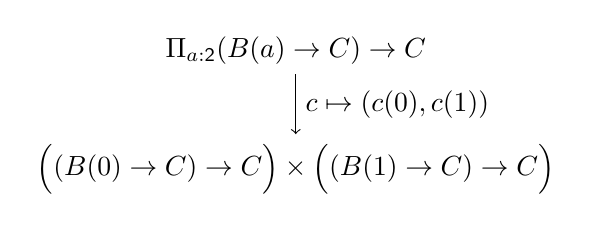
\begin{tikzpicture}
\node (N0) at (0,12) {$\prd{a:\Bool} (B(a) \to C) \to C$};
\node (N1) at (0,10.5) {$\Big((B(0) \to C) \to C\Big) \times \Big((B(1) \to C) \to C\Big)$};
\draw[->] (N0) -- node[right]{$c \mapsto (c(0), c(1))$} (N1);
\end{tikzpicture}
\end{center}
Since $B(0) = 0$, the type $B(0) \to C$ is contractible, with center $\lam{b:B(0)} \abort(C,F \; b)$. We thus have an equivalence
\begin{center}
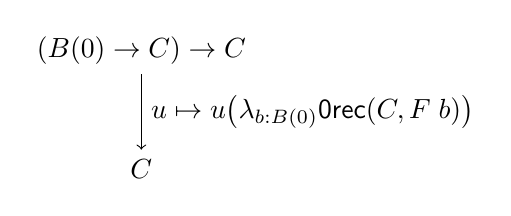
\begin{tikzpicture}
\node (N0) at (0,12) {$(B(0) \to C) \to C$};
\node (N1) at (0,10.5) {$C$};
\draw[->] (N0) -- node[right]{$u \mapsto u\big(\lam{b:B(0)} \abort(C,F \; b)\big)$} (N1);
\end{tikzpicture}
\end{center}
Since $B(1) = 1$, the map $x \mapsto \lam{\_}\; x$ is an equivalence from $C$ to $B(1) \to C$. Thus, we have an equivalence
\begin{center}
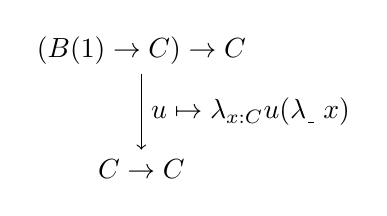
\begin{tikzpicture}
\node (N0) at (0,12) {$(B(1) \to C) \to C$};
\node (N1) at (0,10.5) {$C \to C$};
\draw[->] (N0) -- node[right]{$u \mapsto \lam{x:C} u(\lam{\_} \; x)$} (N1);
\end{tikzpicture}
\end{center}
Putting this all together, we see that the map 
\[ (C,c) \mapsto \Big(C,c\big(0,\lam{b} \abort(C,F \; b)\big),\lam{x:C} c(1, \lam{\_} \; x)\Big)\] 
is an equivalence from $\WAlg_{\UU_i}(A,B)$ to $\NatAlg_{\UU_i}$.
\end{proof}

\begin{lemma}
For any $\X : \WAlg_{\UU_i}(A,B)$ there is an equivalence
\[ \WFibAlgToNatFibAlg_{\UU_j} : \WFibAlg_{\UU_j}(A,B) \; \X \to \NatFibAlg_{\UU_j}(\WAlgToNatAlg_{\UU_i}(\X)) \]
\end{lemma}
\begin{proof}
Let an algebra $(C,c) : \WAlg_{\UU_i}(A,B)$ be given and fix $E : C \to \UU_j$. We have an equivalence
\begin{center}
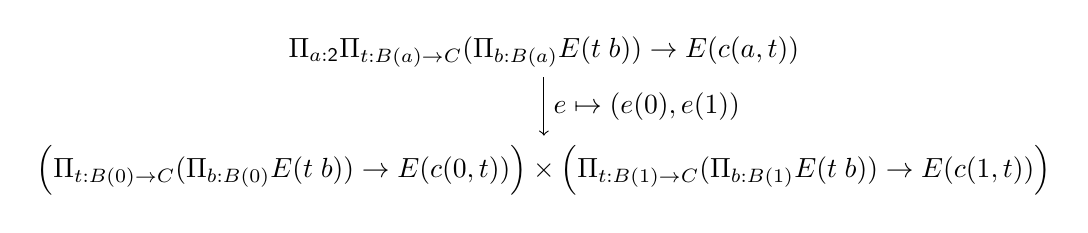
\begin{tikzpicture}
\node (N0) at (0,12) {$\prd{a:\Bool}\prd{t:B(a)\to C} (\prd{b:B(a)} E(t\;b)) \to E(c(a,t))$};
\node (N1) at (0,10.5) {$\Big(\prd{t:B(0)\to C} (\prd{b:B(0)} E(t\;b)) \to E(c(0,t))\Big) \times \Big(\prd{t:B(1)\to C} (\prd{b:B(1)} E(t\;b)) \to E(c(1,t))\Big)$};
\draw[->] (N0) -- node[right]{$e \mapsto (e(0), e(1))$} (N1);
\end{tikzpicture}
\end{center}
Since $B(0) = 0$, the type $B(0) \to C$ is contractible, with center $\lam{b:B(0)} \abort(C,F \; b)$. Likewise, $\prd{b:B(0)} E(\abort(C,F \; b))$ is contractible, with center 
$\lam{b:B(0)} \abort\big(E(\abort(C,F \; b)), F \;b\big)$. We thus have equivalences
\begin{center}
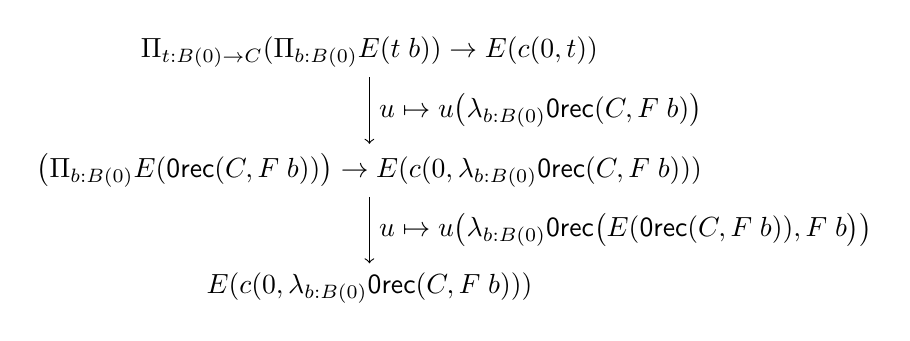
\begin{tikzpicture}
\node (N0) at (0,12) {$\prd{t:B(0)\to C} (\prd{b:B(0)} E(t\;b)) \to E(c(0,t))$};
\node (N1) at (0,10.5) {$\big(\prd{b:B(0)} E(\abort(C,F \; b))\big) \to E(c(0,\lam{b:B(0)} \abort(C,F \; b)))$};
\node (N2) at (0,9) {$E(c(0,\lam{b:B(0)} \abort(C,F \; b)))$};
\draw[->] (N0) -- node[right]{$u \mapsto u\big(\lam{b:B(0)} \abort(C,F \; b)\big)$} (N1);
\draw[->] (N1) -- node[right]{$u \mapsto u\big(\lam{b:B(0)} \abort\big(E(\abort(C,F \; b)), F \;b\big)\big)$} (N2);
\end{tikzpicture}
\end{center}
Since $B(1) = 1$, the map $x \mapsto \lam{\_}\; x$ is an equivalence from $C$ to $B(1) \to C$. Likewise, for any $x:C$ the map $y \mapsto \lam{\_}\; y$  is an equivalence from $E(x)$ to $B(1) \to E(x)$. Thus, we have equivalences
\begin{center}
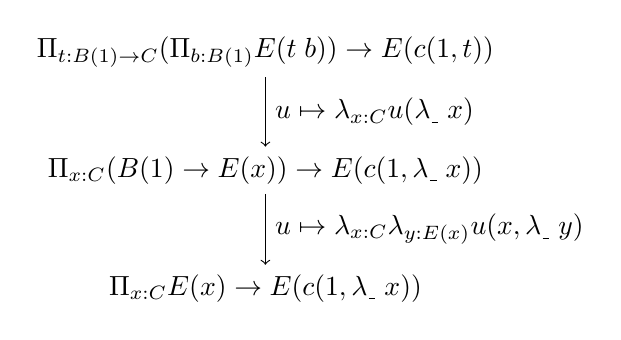
\begin{tikzpicture}
\node (N0) at (0,12) {$\prd{t:B(1)\to C} (\prd{b:B(1)} E(t\;b)) \to E(c(1,t))$};
\node (N1) at (0,10.5) {$\prd{x:C} (B(1) \to E(x)) \to E(c(1,\lam{\_} \; x))$};
\node (N2) at (0,9) {$\prd{x:C} E(x) \to E(c(1,\lam{\_} \; x))$};
\draw[->] (N0) -- node[right]{$u \mapsto \lam{x:C} u(\lam{\_} \; x)$} (N1);
\draw[->] (N1) -- node[right]{$u \mapsto \lam{x:C} \lam{y:E(x)} u(x,\lam{\_} \; y)$} (N2);
\end{tikzpicture}
\end{center}
Putting this all together, we see that the map 
\[ (E,e) \mapsto \Big(E,e\big(0,\lam{b} \abort(C,F \; b), \lam{b} \abort(E(\abort(C,F \; b)), F \;b)\big),\lam{x:C} \lam{y:E(x)} e(1, \lam{\_} \; x, \lam{\_} \; y)\Big)\] 
is an equivalence from $\WFibAlg_{\UU_j}(A,B) \; (C,c)$ to $\NatFibAlg_{\UU_j}(\WAlgToNatAlg_{\UU_i} \; (C,c))$.
\end{proof}

\begin{lemma}
For any $\X : \WAlg_{\UU_i}(A,B)$ and $\Y : \WFibAlg_{\UU_j}(A,B) \; \X$ we have
\[ \WFibHom \; \X \; \Y \;\; \simeq \;\; \NatFibHom \; \big(\WAlgToNatAlg_{\UU_i}(\X)\big) \; \big(\WFibAlgToNatFibAlg_{\UU_j}(\Y)\big) \]
\end{lemma}
\begin{proof}
Let algebras $(C,c) : \WAlg_{\UU_i}(A,B)$ and $(E,e) : \WFibAlg_{\UU_j}(A,B) \; (C,c)$ be given and fix $f : \prd{x:C} E(x)$. We have an equivalence
\begin{center}
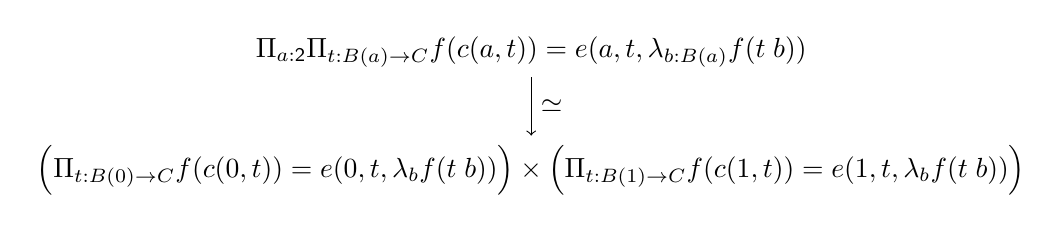
\begin{tikzpicture}
\node (N0) at (0,12) {$\prd{a:\Bool}\prd{t:B(a)\to C} f(c(a,t)) = e(a,t,\lam{b:B(a)} f(t\;b))$};
\node (N1) at (0,10.5) {$\Big(\prd{t:B(0)\to C} f(c(0,t)) = e(0,t,\lam{b} f(t\;b))\Big) \times \Big(\prd{t:B(1)\to C} f(c(1,t)) = e(1,t,\lam{b} f(t\;b))\Big)$};
\draw[->] (N0) -- node[right]{$\simeq$} (N1);
\end{tikzpicture}
\end{center}
Since $B(0) = 0$, the type $B(0) \to C$ is contractible, with center $\lam{b:B(0)} \abort(C,F \; b)$. Furthermore, since all functions out of $\zero$ are equal, we have
\[\lam{b} f(\abort(C,F \; b)) = \lam{b} \abort(E(\abort(C,F \; b)), F \;b)\] This implies the following equivalences:
\begin{center}
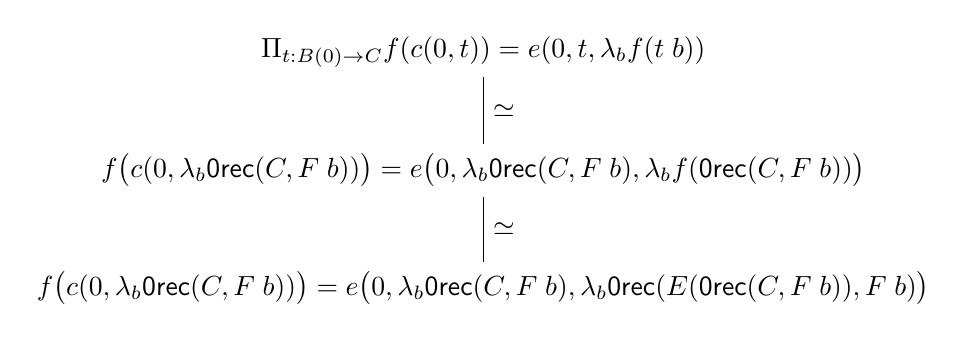
\begin{tikzpicture}
\node (N0) at (0,12) {$\prd{t:B(0)\to C} f(c(0,t)) = e(0,t,\lam{b} f(t\;b))$};
\node (N1) at (0,10.5) {$f\big(c(0,\lam{b} \abort(C,F \; b))\big) = e\big(0,\lam{b} \abort(C,F \; b),\lam{b} f(\abort(C,F \; b))\big)$};
\node (N2) at (0,9) {$f\big(c(0,\lam{b} \abort(C,F \; b))\big) = e\big(0,\lam{b} \abort(C,F \; b),\lam{b} \abort(E(\abort(C,F \; b)), F \;b)\big)$};
\draw[-] (N0) -- node[right]{$\simeq$} (N1);
\draw[-] (N1) -- node[right]{$\simeq$} (N2);
\end{tikzpicture}
\end{center}
Since $B(1) = 1$, the map $x \mapsto \lam{\_}\; x$ is an equivalence from $C$ to $B(1) \to C$. Thus, we have an equivalence
\begin{center}
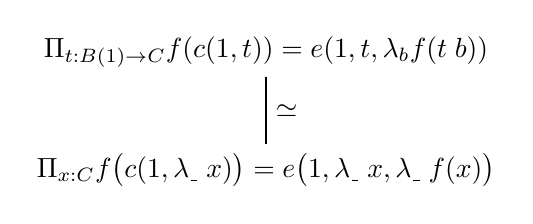
\begin{tikzpicture}
\node (N0) at (0,12) {$\prd{t:B(1)\to C} f(c(1,t)) = e(1,t,\lam{b} f(t\;b))$};
\node (N1) at (0,10.5) {$\prd{x:C} f\big(c(1,\lam{\_} \; x)\big) = e\big(1,\lam{\_} \; x,\lam{\_} \; f(x)\big)$};
\draw[-] (N0) -- node[right]{$\simeq$} (N1);
\end{tikzpicture}
\end{center}
This finishes the proof.
\end{proof}

\begin{corollary}
For any $\X : \WAlg_{\UU_i}(A,B)$ and $\Y : \WAlg_{\UU_j}(A,B)$ we have
\[ \WHom \; \X \; \Y \;\; \simeq \;\; \NatHom \; \big(\WAlgToNatAlg_{\UU_i}(\X)\big) \; \big(\WAlgToNatAlg_{\UU_j}(\Y)\big) \]
\end{corollary}

\begin{corollary}
For any $\X : \NatAlg_{\UU_i}$ we have
\begin{alignat*}{4}
& \HasNatRec_{\UU_j}(\X) & \;\; \simeq \;\; & \HasWRec_{\UU_j}(\WAlgToNatAlg_{\UU_i}^{-1}(\X)) \\
& \HasNatInd_{\UU_j}(\X) & \;\; \simeq \;\; & \HasWInd_{\UU_j}(\WAlgToNatAlg_{\UU_i}^{-1}(\X)) \\
& \HasNatRecUniq_{\UU_j}(\X) &  \simeq \;\; & \HasWRecUniq_{\UU_j}(\WAlgToNatAlg_{\UU_i}^{-1}(\X)) \\
& \HasNatIndUniq_{\UU_j}(\X) & \simeq \;\; &  \HasWIndUniq_{\UU_j}(\WAlgToNatAlg_{\UU_i}^{-1}(\X)) \\
& \IsNatHInit_{\UU_j}(\X) & \simeq \;\; & \IsWHInit_{\UU_j}(\WAlgToNatAlg_{\UU_i}^{-1}(\X))
\end{alignat*}
\end{corollary}

\begin{corollary}\label{lem:NatMainInt}
In $\Hint$, the following conditions on an algebra $\X : \NatAlg_{\UU_i}$ are equivalent:
\begin{enumerate}
\item $\X$ satisfies the induction principle on the universe $\UU_j$
\item $\X$ satisfies the recursion and recursion uniqueness principles on the universe $\UU_j$
\item $\X$ is homotopy-initial on the universe $\UU_j$  
\end{enumerate}
for $j \geq i$. In other words, we have \[ \HasNatInd_{\UU_j}(\X)  \;\; \simeq \;\; \HasNatRec_{\UU_j}(\X) \times \HasNatRecUniq_{\UU_j}(\X) \;\; \simeq \;\; \IsNatHInit_{\UU_j}(\X) \]
provided $j \geq i$. Furthermore, all 3 conditions are mere propositions.
\end{corollary}

We can thus characterize the type $\nat$ using the universal property of initiality as follows.
\begin{corollary}\label{lem:NatInitInt}
In $\Hint$ with natural numbers, the algebra $(\nat,\z,\suc(-)) : \NatAlg_{\UU_0}$ is homotopy-initial on any universe $\UU_j$.
\end{corollary}

\begin{corollary}\label{lem:NatCharInt}
In $\Hint$ extended with an algebra $\X : \NatAlg_{\UU_0}$ which is homotopy-initial on any universe $\UU_j$, the type $\nat$ with propositional computation rules is definable. 
\end{corollary}
\begin{proof}
We have an algebra $\cdot \vdash \X : \NatAlg_{\UU_0}$ such that for any $j$, there exists a term $\cdot \vdash h_j  : \IsNatHInit_{\UU_j}(\X)$. Since the requirement $j \geq 0$ always holds, Cor.~\ref{lem:NatMainInt} implies that for any $j$, we have a term $\cdot \vdash r_j : \HasNatInd_{\UU_j}(\X)$. This implies that the type $\nat$ with propositional computation rules is definable.
\end{proof}






\section{Acknowledgements}

We would like to thank Vladimir Voevodsky and Michael Warren for helpful discussions
on the subject of this paper. In particular, Vladimir Voevodsky suggested a simplification of the 
proof that the rules for homotopical W-types imply h-initiality.

Steve Awodey gratefully acknowledges the support of the National Science Foundation, Grant DMS-1001191
 and the Air Force OSR, Grant 11NL035.
Nicola Gambino is grateful for the support of the Institute for Advanced Study, where
he worked on this project. This work was supported by the National Science Foundation 
under agreement No.\ DMS-0635607. Any opinions, findings and conclusions or recommendations
expressed in this material are those of the authors and do not necessarily reflect the views of
the National Science Foundation.
Kristina Sojakova is grateful for the support of CyLab at Carnegie
Mellon under grants DAAD19-02-1-0389 and W911NF-09-1-0273 from the Army
Research Office.



\bibliographystyle{plain}

\bibliography{references}
                        


\end{document}